% ============================================================
%  FR Power Thesis — Main Document
%  EDHEC MSc Data Analysis & AI
%  Compiler: pdflatex (Overleaf compatible)
% ============================================================

\documentclass[12pt, a4paper, oneside]{report}

% ── Encoding & language ──────────────────────────────────────
\usepackage[T1]{fontenc}
\usepackage[utf8]{inputenc}
\usepackage[english]{babel}

% ── Typography ───────────────────────────────────────────────
\usepackage{lmodern}
\usepackage{microtype}
\usepackage{setspace}
\onehalfspacing

% ── Page layout ──────────────────────────────────────────────
\usepackage[
  top=2.5cm, bottom=2.5cm,
  left=3.0cm, right=2.5cm
]{geometry}

% ── Mathematics ──────────────────────────────────────────────
\usepackage{amsmath, amssymb, amsthm}

% ── Figures & tables ─────────────────────────────────────────
\usepackage{graphicx}
\usepackage{booktabs}
\usepackage{tabularx}
\usepackage{multirow}
\usepackage{array}
\usepackage{float}
\usepackage[font=small, labelfont=bf, justification=centering]{caption}
\usepackage{subcaption}

% ── Colours ──────────────────────────────────────────────────
\usepackage[dvipsnames]{xcolor}
\definecolor{edhec}{RGB}{0, 62, 126}
\definecolor{accent}{RGB}{46, 95, 163}

% ── Headers & footers ────────────────────────────────────────
\usepackage{fancyhdr}
\pagestyle{fancy}
\fancyhf{}
\fancyhead[L]{\small\textit{\leftmark}}
\fancyhead[R]{\small\textit{EDHEC MSc Data Analysis \& AI}}
\fancyfoot[C]{\thepage}
\renewcommand{\headrulewidth}{0.4pt}
\renewcommand{\footrulewidth}{0pt}

% ── Section formatting ───────────────────────────────────────
\usepackage{titlesec}
\titleformat{\chapter}[display]
  {\normalfont\Large\bfseries\color{edhec}}
  {\chaptertitlename\ \thechapter}{12pt}{\Huge}
\titlespacing*{\chapter}{0pt}{-20pt}{30pt}

\titleformat{\section}
  {\normalfont\large\bfseries\color{accent}}
  {\thesection}{1em}{}
\titleformat{\subsection}
  {\normalfont\normalsize\bfseries}
  {\thesubsection}{1em}{}

% ── Hyperlinks ───────────────────────────────────────────────
\usepackage[
  colorlinks=true,
  linkcolor=edhec,
  citecolor=accent,
  urlcolor=accent,
  bookmarks=true,
  pdfauthor={Leo Cambreleng and Lyam Oumedjeber},
  pdftitle={The Role of Weather in French Day-Ahead Electricity Price Forecasting}
]{hyperref}

% ── Bibliography ─────────────────────────────────────────────
\usepackage[round, authoryear, sort]{natbib}

% ── Code listings ────────────────────────────────────────────
\usepackage{listings}
\lstset{
  basicstyle=\ttfamily\small,
  breaklines=true,
  frame=single,
  backgroundcolor=\color{gray!8}
}

% ── Embedded file attachment ─────────────────────────────────
\usepackage{attachfile2}

% ── Misc ─────────────────────────────────────────────────────
\usepackage{enumitem}
\usepackage{csquotes}
\usepackage{acronym}
\usepackage{appendix}

% ── Path to figures ──────────────────────────────────────────
\graphicspath{{figures/}}

% ============================================================
\begin{document}

% ── Title page ───────────────────────────────────────────────
\begin{titlepage}
  \centering
  \vspace*{1cm}

  {\color{edhec}\rule{\linewidth}{2pt}}
  \vspace{0.5cm}

  {\LARGE\bfseries\color{edhec}
    The Role of Weather in French\\[6pt]
    Day-Ahead Electricity Price Forecasting:\\[6pt]
    A Random Forest Approach
  \par}

  \vspace{0.5cm}
  {\color{edhec}\rule{\linewidth}{1pt}}
  \vspace{1.5cm}

  {\large Master's Thesis\\[4pt]
   MSc Data Analysis \& AI\\[4pt]
   EDHEC Business School}

  \vspace{2cm}

  {\large\bfseries Leo Cambreleng}\\[6pt]
  {\normalsize leo.cambreleng@edhec.com}

  \vspace{1cm}

  {\large\bfseries Lyam Oumedjeber}\\[6pt]
  {\normalsize lyam.oumedjeber@edhec.com}

  \vspace{2cm}

  {\normalsize Advisor: Prof.\ Milos Vulanovic\\[4pt]
   EDHEC Business School}

  \vspace{2cm}

  {\large May 2026}

  \vfill
  {\color{edhec}\rule{\linewidth}{2pt}}
\end{titlepage}

% ── EDHEC mandatory declarations ─────────────────────────────
\thispagestyle{empty}
\vspace*{3cm}
\begin{center}
  \textit{``EDHEC Business School does not express approval or disapproval concerning the opinions given in this paper which are the sole responsibility of the authors.''}
\end{center}

\vspace{2cm}

\noindent\textit{``I certify that: the Master Project being submitted for examination is our own research, the data and results presented are genuine and actually obtained by us during the conduct of the research and that we have properly acknowledged using parenthetical indications and a full bibliography all areas where we have drawn on the work, ideas and results of others and that the master project has not been presented to any other examination committee before and has not been published before.''}

\vspace{2cm}
\noindent\textbf{Leo Cambreleng} \hfill \textbf{Lyam Oumedjeber}
\clearpage

% ── Abstract ─────────────────────────────────────────────────
\chapter*{Abstract}
\addcontentsline{toc}{chapter}{Abstract}

This thesis investigates whether weather variables significantly improve
day-ahead electricity price forecasting for the French market (EPEX SPOT
France) using machine learning models. We build a comprehensive dataset
spanning January 2018 to April 2025, combining hourly price and generation
data from the ENTSO-E Transparency Platform with ERA5 reanalysis weather data,
cross-border flow data, and fuel price series (TTF natural gas, ARA coal).

Four models are compared: a na\"{i}ve lag-168h benchmark (Model A), a Random
Forest without weather features (Model B), a Random Forest with full weather
features (Model C), and an XGBoost model with weather features (Model D).
Models are evaluated on two strict out-of-sample test sets: a stable-regime
period (May 2024 -- April 2025, 8,640 hours) and the 2022 energy crisis
(full year 2022, 8,760 hours).

Our central finding is that \textit{the marginal value of weather features
is regime-dependent}. In the stable 2024--25 test period, weather does not
significantly improve forecast accuracy over the enriched fundamental model
(Diebold-Mariano test: $p = 0.572$) — we attribute this to information
redundancy, whereby the RTE load forecast and TTF gas prices already encode
the meteorological signal implicitly. However, in the 2022 energy crisis, the
same test yields $p < 0.001$ (DM statistic $= -13.27$): weather becomes
highly significant when the gas supply shock decouples TTF from local
temperature and nuclear constraints amplify the demand-price relationship.
Both Random Forest models achieve MAE $\approx$ 16.9 EUR/MWh and
R$^2 \approx 0.776$ in the stable period, representing a 49\% reduction in
error over the na\"{i}ve benchmark. A day-ahead directional trading backtest
confirms the economic value of these forecasts, with RF models generating net
profits of approximately 136,700 EUR/MW with a Sharpe ratio of 19.5 and a
maximum drawdown approximately 5.6 times smaller than the na\"{i}ve strategy.

\vspace{1em}
\noindent\textbf{Keywords:} electricity price forecasting, day-ahead market,
EPEX SPOT France, Random Forest, XGBoost, weather features, Diebold-Mariano
test, information redundancy, 2022 energy crisis, trading backtest.

% ── Acknowledgements ─────────────────────────────────────────
\chapter*{Acknowledgements}
\addcontentsline{toc}{chapter}{Acknowledgements}

We would like to thank EDHEC Business School for their guidance throughout this project. We are grateful to RTE (R\'{e}seau de Transport d'Électricit\'{e}) and ENTSO-E for making electricity market data publicly available through the Transparency Platform, and to the Copernicus Climate Change Service for providing open access to ERA5 reanalysis data.

\medskip
\noindent\textit{Transparency note on AI tools:} This thesis was developed with assistance from AI language model tools (Claude, Anthropic) for writing support, literature structuring, and code review. All analytical decisions, model choices, experimental design, and interpretations of results are the authors' own.

% ── TOC ──────────────────────────────────────────────────────
\tableofcontents
\listoffigures
\listoftables

% ── Acronyms ─────────────────────────────────────────────────
\chapter*{List of Acronyms}
\addcontentsline{toc}{chapter}{List of Acronyms}
\begin{acronym}
  \acro{DA}{Day-Ahead}
  \acro{DM}{Diebold-Mariano}
  \acro{ENTSO-E}{European Network of Transmission System Operators for Electricity}
  \acro{ETS}{Emissions Trading System}
  \acro{EUA}{European Union Allowance}
  \acro{HDD}{Heating Degree Days}
  \acro{CDD}{Cooling Degree Days}
  \acro{CSS}{Clean Spark Spread}
  \acro{CDS}{Clean Dark Spread}
  \acro{MAE}{Mean Absolute Error}
  \acro{RMSE}{Root Mean Square Error}
  \acro{sMAPE}{Symmetric Mean Absolute Percentage Error}
  \acro{MDD}{Maximum Drawdown}
  \acro{MDI}{Mean Decrease in Impurity}
  \acro{RF}{Random Forest}
  \acro{RTE}{R\'{e}seau de Transport d'Électricit\'{e}}
  \acro{TSO}{Transmission System Operator}
  \acro{WSI}{Weather Stress Index}
\end{acronym}

% ── Chapters ─────────────────────────────────────────────────
% ============================================================
%  Chapter 1 — Introduction
% ============================================================
\chapter{Introduction}
\label{chap:intro}

\section{Context and Motivation}

Electricity markets have undergone a fundamental transformation over the past three decades. The progressive liberalisation of European energy markets, accelerated by successive EU directives from 1996 onwards, replaced vertically integrated state monopolies with competitive wholesale markets in which prices are determined by the interaction of supply and demand. In France, the day-ahead electricity market operates through EPEX SPOT, where participants submit bids and offers for each hour of the following day, with a single clearing price determined by a batch auction that closes at 12:00 CET.

The resulting price series is among the most complex in quantitative finance. Unlike commodity prices, electricity cannot be economically stored at scale, which forces supply and demand into instantaneous equilibrium at every moment. The consequence is a price process characterised by extreme volatility, sharp intraday seasonality, strong weekly periodicity, and irregular price spikes that can reach several thousand euros per megawatt-hour during scarcity episodes. The French market adds a layer of specificity: with approximately 63 GW of installed nuclear capacity representing roughly 70\% of annual electricity production \citep{rte2023}, the availability of the nuclear fleet is a primary determinant of price levels. In parallel, France's residential heating stock is predominantly electric, creating a thermosensitivity of approximately 2.4 GW per degree Celsius in winter \citep{rte2024} — the highest in Europe.

Accurate forecasting of day-ahead prices is therefore not merely an academic exercise. It is a critical input for energy suppliers setting customer tariffs, for industrial consumers optimising consumption schedules, for renewables producers valuing flexibility options, and for traders positioning in forward markets. A one euro per megawatt-hour improvement in forecast accuracy over a 100 MW portfolio translates to approximately 876,000 EUR in annual value capture — motivating sustained interest in more accurate models.

\section{Research Question}

This thesis addresses the following central question:

\begin{quote}
\textit{Do weather variables significantly improve the accuracy of day-ahead
electricity price forecasts for the French market, and does their contribution
depend on the market regime?}
\end{quote}

This question is decomposed into four sub-questions:

\begin{enumerate}
  \item Can machine learning models (Random Forest, XGBoost) substantially
  outperform a na\"{i}ve statistical benchmark on French day-ahead prices?
  \item Does the addition of meteorological features (temperature, wind speed,
  solar radiation, Heating Degree Days, Weather Stress Index) produce a
  statistically significant improvement over a model built on market
  fundamentals alone — and is this result stable across market regimes?
  \item Does the marginal value of weather features differ between a stable
  market regime (2024--25) and an extreme-stress regime (2022 energy crisis),
  and what structural mechanisms explain any difference?
  \item Can the predictive improvement of these models be translated into
  economically meaningful returns through a day-ahead directional trading
  strategy with realistic transaction costs?
\end{enumerate}

\section{Contribution}

This thesis makes four contributions to the electricity price forecasting
literature:

\begin{itemize}
  \item \textbf{Comprehensive French dataset:} We assemble and publish a
  reproducible dataset spanning 2018--2025 that combines ENTSO-E generation
  and load data, ERA5 reanalysis weather data, cross-border flow data, and
  fuel price series. To our knowledge, this is one of the most complete
  publicly-sourced datasets for the French day-ahead market.

  \item \textbf{Rigorous weather ablation study with regime comparison:}
  We design a four-model experiment (A/B/C/D) isolating the marginal
  contribution of weather features using a Diebold-Mariano test with
  Harvey-Leybourne-Newbold correction, applied to two out-of-sample periods.
  Our key finding is that weather is statistically non-significant in a stable
  regime ($p = 0.572$) but highly significant in the 2022 energy crisis
  ($p < 0.001$, DM $= -13.27$). We explain this regime-dependence through
  the \textit{information redundancy hypothesis}: in normal conditions, the
  RTE load forecast and TTF gas prices subsume the weather signal; in crisis
  conditions, the gas supply shock breaks this redundancy.

  \item \textbf{2022 energy crisis as a natural experiment:} We exploit the
  2022 French-European energy crisis — characterised by simultaneously low
  nuclear availability ($\approx$40\%) and extreme gas prices — as a stress
  test of the weather redundancy hypothesis. This provides the first formal
  evaluation of regime-dependence in the weather-price relationship for the
  French market.

  \item \textbf{Day-ahead executable trading backtest:} We implement a
  directional trading strategy using an economically coherent signal design
  grounded in the actual mechanics of the EPEX SPOT day-ahead auction, with
  dead-band filtering and three realistic transaction cost scenarios drawn
  from the 2024 EPEX fee schedule.
\end{itemize}

\section{Structure of the Thesis}

The remainder of this thesis is organised as follows. Chapter~\ref{chap:lit} reviews the literature on electricity price forecasting, covering both statistical and machine learning approaches. Chapter~\ref{chap:data} describes the data sources, feature engineering process, and exploratory analysis. Chapter~\ref{chap:model} presents the modelling framework, results, and statistical tests. Chapter~\ref{chap:backtest} introduces the trading backtest and its results. Chapter~\ref{chap:discussion} discusses the findings, limitations, and extensions. Chapter~\ref{chap:conclusion} concludes.

All code, data pipelines, trained models, and figures are available in the project repository at \url{https://github.com/leogthub/fr-power-thesis}.

% ============================================================
%  Chapter 2 — Literature Review
% ============================================================
\chapter{Literature Review}
\label{chap:lit}

\section{Overview of Electricity Price Forecasting}

The electricity price forecasting (EPF) literature has expanded rapidly since
market liberalisation began in the 1990s. \citet{weron2014} provides the
definitive survey, classifying approaches into five families: (1) multi-agent
models, (2) fundamental models, (3) reduced-form stochastic models,
(4) statistical models, and (5) computational intelligence models. The survey
covers over two decades of research and remains the standard reference for
the field, identifying that no single method dominates across all markets and
horizons, and that the most practically useful improvements typically come from
better feature engineering rather than more complex model architectures.
More recently, \citet{nowotarski2018} document the shift towards probabilistic
forecasting and machine learning methods, arguing that ensemble combination
of diverse forecasting approaches consistently outperforms individual models.

The field has converged on several stylised facts about electricity price
dynamics: (1) prices exhibit multi-frequency seasonality (intraday, weekly,
annual); (2) the distribution is heavily right-skewed with non-trivial negative
mass; (3) extreme price spikes are driven by fundamental supply-demand
imbalances rather than by speculative dynamics; and (4) the price-setting
technology shifts across hours and seasons, making the relationship between
fundamentals and prices inherently non-linear. These characteristics motivate
the use of non-linear ensemble methods capable of capturing threshold effects
and interaction terms.

For the purposes of this thesis, we focus on short-term \textit{point}
forecasting at the day-ahead horizon, which remains the most practically
relevant setting for physical market participants who must submit bids to the
EPEX SPOT auction by 12:00 CET each day. The review is structured around three
questions: (1) what methods have been proposed and evaluated? (2) what role
does weather play in these models? and (3) how should models be formally
compared?

\section{Statistical and Econometric Approaches}

Early work on day-ahead price forecasting relied on time-series models adapted
from financial econometrics. Autoregressive models — in particular ARIMA and
its seasonal extensions (SARIMA) — capture the strong autocorrelation structure
of electricity prices but struggle to model the non-linear interactions between
price and its fundamental drivers. GARCH-family models address volatility
clustering \citep{weron2014} but are ill-suited to the extreme price spikes
that characterise electricity markets, where the distribution of returns has
much heavier tails than financial asset returns, including a non-trivial mass
of negative observations \citep{fanone2013}.

The mean-reversion and jump-diffusion framework, introduced in the commodity
pricing literature, is better able to capture the spike-and-reversion behaviour
of electricity prices. However, these structural models typically require
numerical methods for calibration and are difficult to extend to include
exogenous weather or fundamental variables, limiting their usefulness when
the research objective is to quantify the marginal contribution of individual
predictors.

Factor models and regularised regression represent an important middle ground.
\citet{maciejowska2016} apply Factor Quantile Regression Averaging to
day-ahead prices across European markets, combining multiple linear
specifications through optimal weights. Critically, \citet{uniejewski2019}
demonstrate that automated variable selection using LASSO regularisation applied
to a rich set of price lags and calendar variables achieves competitive
performance relative to more complex non-linear models, even on markets with
high renewable penetration. This result — that well-specified linear models
with carefully chosen price lags can be surprisingly competitive — is directly
relevant to our finding that weather adds negligible marginal value once price
lags and fundamental variables are included. The common thread is that the
predictive information in electricity prices is highly concentrated in recent
price history: any additional variable, whether weather-based or
fundamental-based, must provide information \textit{not already present} in
recent prices to justify its inclusion.

\section{Machine Learning Approaches}

The application of machine learning to electricity price forecasting has
accelerated since the mid-2010s, driven by the increasing availability of
high-resolution data and cheap computational resources. \citet{aggarwal2009}
provide an early review, while \citet{lago2018} offer an empirical comparison
of deep learning architectures (LSTM, CNN) against traditional benchmarks on
European day-ahead markets, finding that deep learning improves on ARIMA but
not consistently over well-tuned tree ensembles.

The most systematic evaluation of machine learning methods for EPF is provided
by \citet{lago2021}, who benchmark 27 algorithms across 12 European electricity
markets using a standardised open-source evaluation framework. Their key
finding is that no algorithm consistently dominates: the best-performing method
varies by market and time period, and the margin of improvement from complex
deep learning over simpler tree-based methods is often statistically
insignificant once proper Diebold-Mariano testing is applied. For the French
market specifically, \citet{lago2021} report benchmark MAE values in the range
of 10--25 EUR/MWh under stable market conditions, which provides the reference
frame against which our results (MAE $\approx$ 16.94 EUR/MWh in May 2024 --
April 2025) should be interpreted. The authors explicitly recommend that EPF
papers adopt DM testing as standard practice for model comparison, a
recommendation we follow throughout Chapter~\ref{chap:model}.

\textbf{Tree-based ensemble methods} — Random Forests \citep{breiman2001} and
Gradient Boosted Trees (including XGBoost, \citealt{chen2016}) — have proven
particularly well-suited to the EPF problem for several reasons. First, they
handle non-linear interactions between weather, calendar, and fundamental
variables without requiring manual feature transformations. Second, they are
robust to outliers and near-zero prices, which are frequent in liberalised
markets and create difficulties for methods that rely on symmetric loss
functions. Third, tree ensembles provide built-in feature importance measures
(Mean Decrease in Impurity for Random Forests) that offer interpretable
insights into price drivers, a property highly valued by market participants
who must justify their models to risk committees. \citet{tschora2022} confirm in a
recent comparative study on European day-ahead markets that gradient boosted trees
remain competitive with neural network architectures on EPF tasks when sample sizes
are moderate ($n < 100{,}000$ hourly observations), as in our setting.

\citet{ziel2018} compare univariate and multivariate forecasting frameworks on
European day-ahead markets and find that multivariate models incorporating
load, generation, and cross-border flows outperform univariate price-only
models, supporting the use of fundamental variables in our feature matrix.
A consistent finding across the ML literature is that price lags dominate
feature importance rankings when included in the feature matrix \citep{lago2021,
uniejewski2019}. This is consistent with the strong autocorrelation structure
of electricity prices and the difficulty of improving over recent price history
as a predictor. Our results — where the 24-hour price lag accounts for
approximately 22\% of total MDI importance — are in line with this consensus.

\section{Weather as a Driver of Electricity Prices}

The causal pathway from weather to electricity prices is well-established in
the fundamental literature. Temperature affects demand through heating (in
winter) and cooling (in summer). Wind speed determines the output of wind
generators, which can set the marginal cost to zero when in excess, driving
prices downward. Solar irradiance compresses midday prices during
high-penetration periods, a phenomenon known as the ``solar merit order
effect''. Precipitation affects hydro reservoir levels, with droughts leading
to higher thermal generation and higher prices.

\citet{staffell2016} document the strong correlation between wind speed and
wind generation output (approximately cubic relationship), which underlies our
\textit{wind power proxy} feature.

In the French market specifically, the thermosensitivity is unusually high by
European standards. \citet{rte2023} report that each degree Celsius below
17\textdegree C increases peak demand by approximately 2.4 GW — a consequence
of the high penetration of electric heating (over 30\% of French households).
This motivates the use of 17\textdegree C as the Heating Degree Day threshold
throughout this thesis, consistent with RTE's own operational methodology and
higher than the 15\textdegree C threshold used in Germany.

However, the literature has increasingly recognised that weather effects on
electricity prices may be \textit{indirect} rather than direct — transmitted
through other observable variables. If electricity prices are primarily set by
the marginal cost of gas-fired generation, and if gas prices themselves respond
to pan-European heating demand, then a model including TTF gas prices may
already capture the meteorological signal without explicit weather features.
This indirect transmission channel is the foundation of our information
redundancy hypothesis.

The 2021--2023 European energy crisis provides a natural experiment on this
hypothesis. The simultaneous withdrawal of Russian pipeline gas supply and
France's historically low nuclear availability (reaching $\approx$40\% in
mid-2022 due to corrosion-related maintenance) created a regime in which gas
prices became the dominant driver of electricity prices across Europe. In such
a regime, the direct weather channel — cold temperatures increasing electricity
demand directly — may be more visible above the gas price noise than in normal
market conditions. Testing whether weather features are more informative during
the 2022 crisis than in the 2024--25 normalisation period is a central
contribution of this thesis (Section~\ref{sec:validation2022}).

\section{Diebold-Mariano Testing in Energy Forecasting}

Comparing forecast accuracy across models requires careful statistical
treatment. Informal comparisons based on point estimates of MAE or RMSE can
lead to misleading conclusions when differences are not statistically
significant. The Diebold-Mariano (DM) test \citep{diebold1995} provides a
formal framework for testing the null hypothesis of equal predictive accuracy
between two competing forecasts. The test statistic is based on the difference
in loss functions (here, absolute errors) and accounts for autocorrelation in
the loss differential series via a Newey-West long-run variance estimator
\citep{newbold1993}.

For small samples, \citet{harvey1997} propose a correction factor that adjusts
the DM statistic to better approximate a $t$-distribution, reducing the risk
of over-rejection of the null. We apply this Harvey-Leybourne-Newbold (HLN)
correction throughout our analysis, following best practice in the EPF
literature \citep{weron2014}. \citet{lago2021} explicitly recommend the
DM test with HLN correction as the standard for EPF model comparisons, noting
that many published results that appear significant on point metrics alone are
not statistically significant once proper testing is applied. Adopting this
standard is particularly important for our weather ablation study: the
difference in MAE between our models B and C is only 0.01 EUR/MWh — a
difference that appears negligible on inspection and is confirmed as
statistically insignificant by the DM test ($p = 0.572$).

\section{Gap in the Literature}

Despite the growing body of work on machine learning for electricity price
forecasting, several gaps remain relevant to this thesis:

\begin{enumerate}
  \item \textbf{French market specificity:} Most empirical studies focus on the
  German, Spanish, or Nordic markets, or treat European markets as homogeneous.
  The French market's combination of dominant nuclear share ($\approx$70\% of
  generation in normal conditions), unusually high thermosensitivity, and
  interconnection with multiple neighbours creates a distinct price formation
  mechanism. The 2022 crisis, during which France's nuclear availability fell
  to an unprecedented 40\%, represents a structurally unique episode whose
  impact on the weather-price relationship has not been formally studied in the
  EPF literature.

  \item \textbf{Formal ablation of weather features:} While weather variables
  are routinely included in EPF models, their marginal contribution is rarely
  isolated using a statistically formal test. Most studies either exclude
  weather entirely or include it without testing whether its addition is
  statistically significant relative to a fundamental-only baseline. We address
  this gap with a Diebold-Mariano ablation study that directly tests whether
  ERA5 meteorological variables improve on a model that already includes load
  forecasts, fuel prices, and nuclear availability.

  \item \textbf{Regime-dependence of the weather contribution:} No study, to
  our knowledge, explicitly tests whether the marginal contribution of weather
  variables varies across market regimes (crisis vs.\ normal). Our design,
  which evaluates Models B vs C on both the 2024--25 stable period and the 2022
  crisis period using the same DM testing framework, directly addresses this gap
  and produces our most novel empirical finding.

  \item \textbf{Economic value evaluation:} Most studies evaluate models on
  statistical metrics alone. We extend the analysis to an executable day-ahead
  trading backtest with realistic transaction costs and a dead-band filter
  (Chapter~\ref{chap:backtest}), linking statistical accuracy to economic value
  and providing a practitioner-relevant assessment of model quality.
\end{enumerate}

% ============================================================
%  Chapter 3 — Data and Feature Engineering
% ============================================================
\chapter{Data and Feature Engineering}
\label{chap:data}

\section{Data Sources}

Our dataset combines four primary sources, covering the period January 2018 to April 2025 at hourly resolution, yielding approximately 64,000 observations before feature construction.

\subsection{ENTSO-E Transparency Platform}

The European Network of Transmission System Operators for Electricity (ENTSO-E) makes hourly data publicly available through its Transparency Platform \citep{entsoe2024}. We retrieve the following series for France (bidding zone \texttt{10YFR-RTE------C}):

\begin{itemize}
  \item \textbf{Day-ahead prices} (EUR/MWh): the clearing price of the EPEX SPOT France day-ahead auction, which constitutes our forecasting target.
  \item \textbf{Actual total load} and \textbf{load forecast} (MW): the TSO's hourly load forecast, published the day before delivery, serves as a key predictor of demand pressure.
  \item \textbf{Actual generation by source} (MW): nuclear, gas, run-of-river hydro, reservoir hydro, solar, and onshore wind.
  \item \textbf{Cross-border physical flows} (MW): net hourly flows between France and its four main interconnected neighbours — Germany, Spain, the United Kingdom, and Belgium. These flows reflect relative price differentials and capacity constraints across the European internal energy market.
\end{itemize}

Data are retrieved programmatically using the \texttt{entsoe-py} Python library with the official ENTSO-E API key. All timestamps are converted to UTC+1 (Europe/Paris) and aligned on a consistent hourly index.

\subsection{ERA5 Reanalysis Weather Data}

Meteorological variables are sourced from the ERA5 reanalysis dataset produced by the European Centre for Medium-Range Weather Forecasts (ECMWF) through the Copernicus Climate Change Service \citep{hersbach2020}. ERA5 provides hourly estimates of atmospheric variables on a 0.25$^{\circ} \times 0.25^{\circ}$ grid, covering the globe from 1940 to present.

We retrieve the following variables for a bounding box covering metropolitan France (41--51$^{\circ}$N, -5--10$^{\circ}$E) and compute spatial means weighted by grid area:

\begin{itemize}
  \item 2-metre air temperature (\textdegree C)
  \item 10-metre wind speed (m/s)
  \item Surface solar irradiance (W/m$^2$, derived from surface net solar radiation)
  \item Total precipitation (m/h)
\end{itemize}

Data are downloaded month-by-month using the \texttt{cdsapi} library to avoid request size limitations, then concatenated and temporally aligned with the ENTSO-E series.

\subsection{Fuel Prices}

Fuel prices are retrieved from public market data sources:

\begin{itemize}
  \item \textbf{TTF natural gas} (EUR/MWh): the Title Transfer Facility day-ahead price, the European gas benchmark. TTF prices are the primary determinant of the marginal cost of gas-fired generation, which is frequently the price-setting technology in France outside nuclear baseload hours.
  \item \textbf{ARA coal} (EUR/tonne): the price of thermal coal delivered to Amsterdam-Rotterdam-Antwerp. Together with EU ETS carbon allowance costs, coal prices determine the Clean Dark Spread and the relative competitiveness of coal and gas-fired generation. EU ETS carbon allowance prices (EUA) are not retrieved as a standalone feature in this study: their incremental price signal is largely embedded in the TTF-coal spread, and the two fuel price variables together capture the marginal-cost information relevant for gas and coal dispatch. Omitting EUA is a limitation acknowledged in Chapter~\ref{chap:discussion}.
\end{itemize}

\subsection{Price Statistics}

Figure~\ref{fig:price_series} shows the full price series from 2018 to 2025. The period exhibits three distinct regimes: a pre-crisis period (2018--2021) with prices typically between 20--80 EUR/MWh; the energy crisis of 2021--2023, during which French prices reached historical extremes above 1,000 EUR/MWh driven by the simultaneous Russian gas supply disruption and the historically low nuclear availability due to corrosion-related maintenance shutdowns; and a normalisation phase from 2023 onwards as gas prices declined and nuclear availability recovered toward 75--80\%.

\begin{figure}[H]
  \centering
  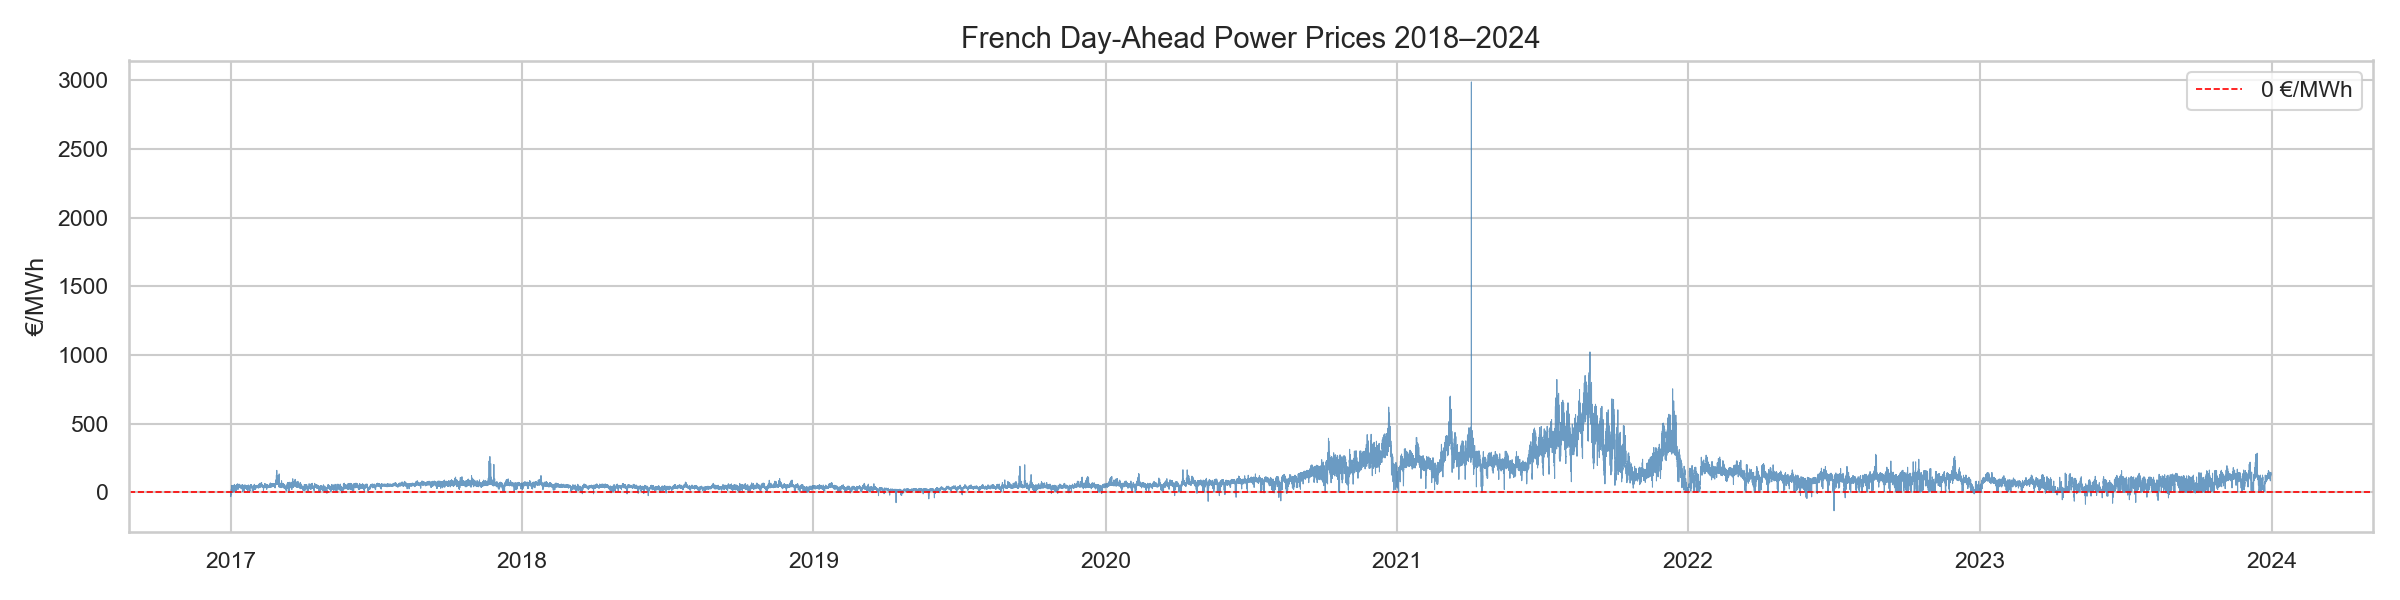
\includegraphics[width=\textwidth]{price_series_full.png}
  \caption{French day-ahead electricity prices (EUR/MWh), January 2018 -- April 2025. The 2022 energy crisis produced historically extreme prices, driven by the simultaneous gas supply shock and low nuclear availability.}
  \label{fig:price_series}
\end{figure}

The distribution of hourly prices is heavily right-skewed with a non-trivial mass of negative observations (Figure~\ref{fig:price_dist}). Negative prices occur when inflexible generators (nuclear, wind) are constrained to run and cannot be economically curtailed, resulting in producers paying consumers to absorb excess generation.

\begin{figure}[H]
  \centering
  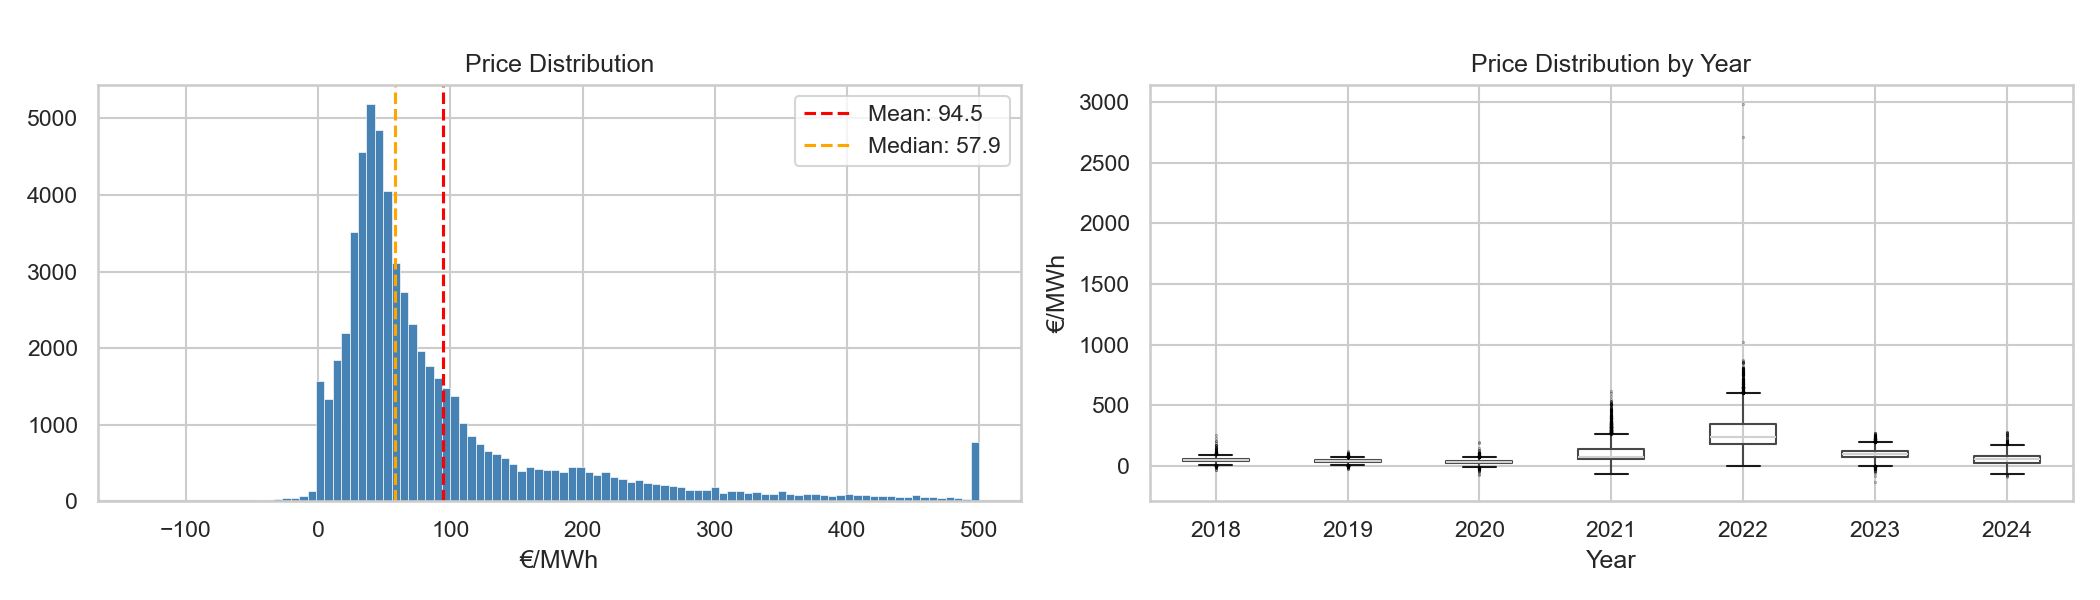
\includegraphics[width=0.9\textwidth]{price_distribution.png}
  \caption{Distribution of hourly day-ahead prices (left) and proportion of negative-price hours by year (right). Negative prices account for approximately 3--8\% of hours in recent years.}
  \label{fig:price_dist}
\end{figure}

The strong seasonality at multiple frequencies is apparent in Figure~\ref{fig:price_heatmap}, which shows the average price by hour of day and month of year. Winter morning and evening peaks, summer midday price compressions from solar generation, and the consistent week/weekend differential are all visible.

\begin{figure}[H]
  \centering
  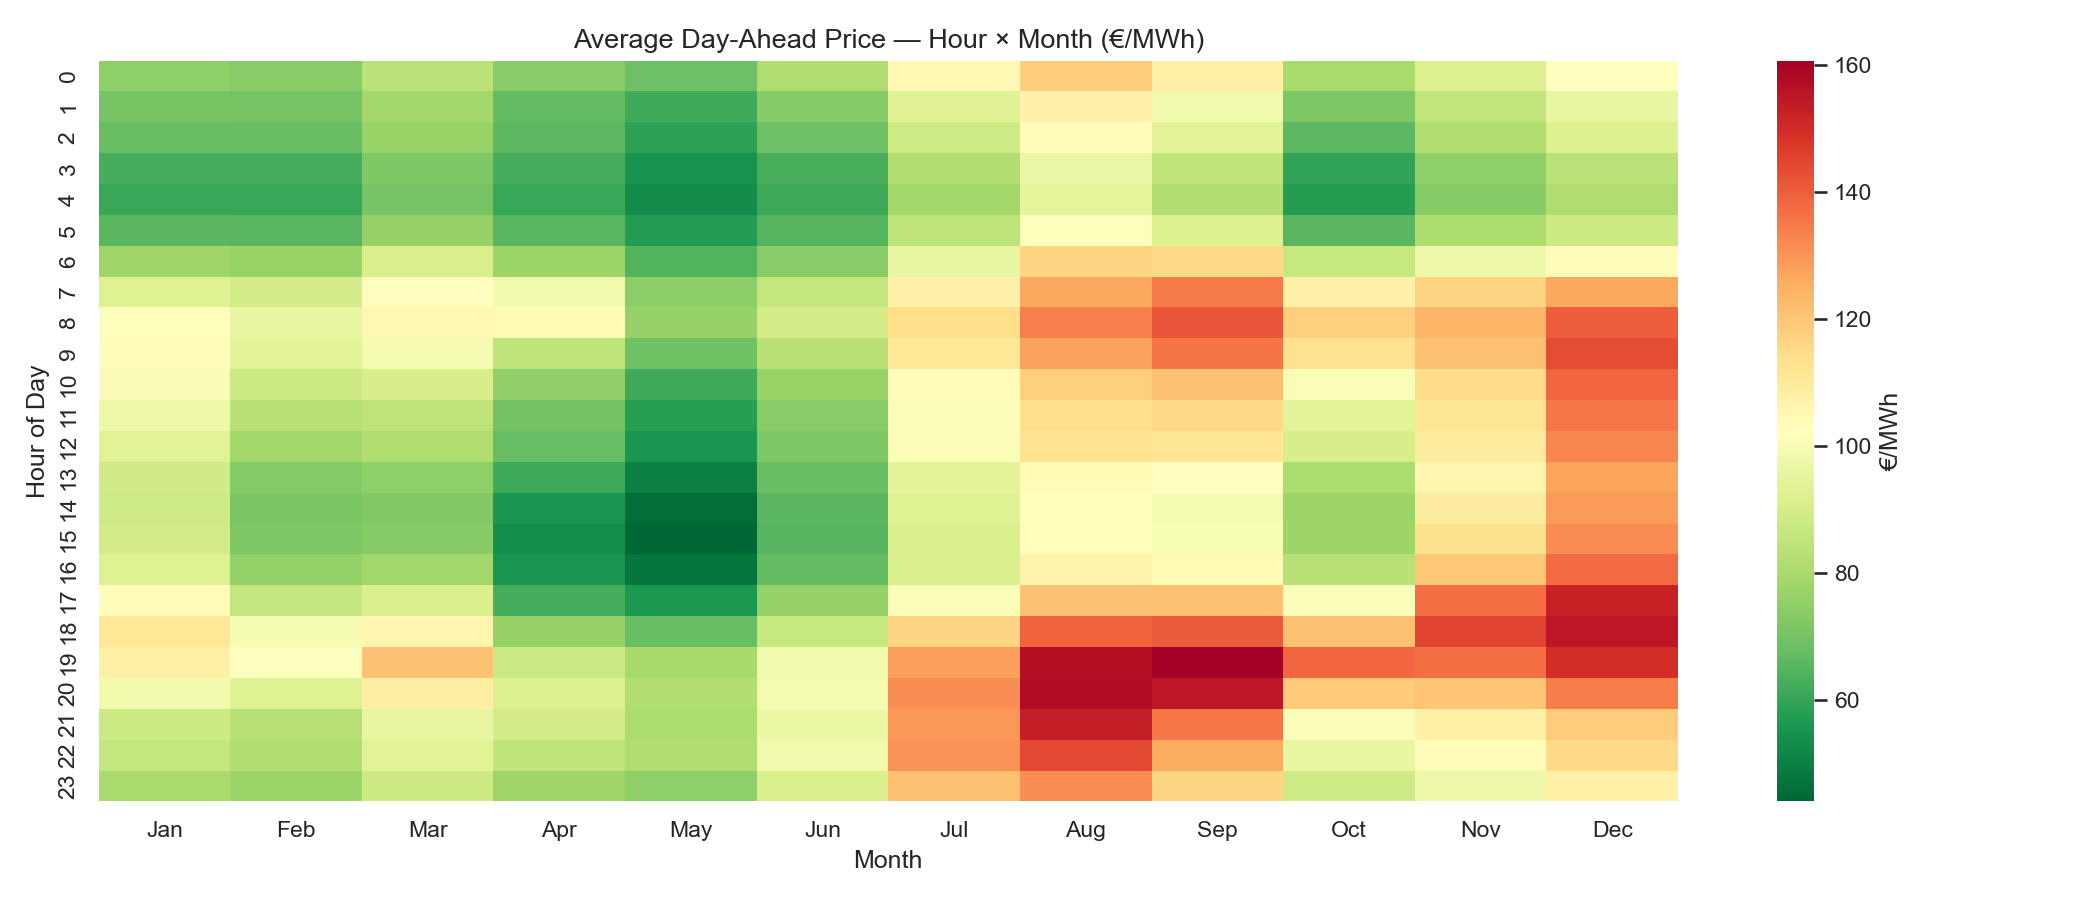
\includegraphics[width=\textwidth]{price_heatmap_hour_month.png}
  \caption{Average hourly price by hour of day and month of year (2018--2025). Dark shading indicates high prices; winter peak hours (07:00--09:00, 18:00--20:00) are systematically elevated.}
  \label{fig:price_heatmap}
\end{figure}

\section{Feature Engineering}
\label{sec:features}

From the raw data sources described above, we construct 35 features organised into five categories. The full list is provided in Appendix~\ref{app:features}; we describe the most methodologically significant features here.

\subsection{Calendar Features}

Calendar variables capture the deterministic seasonality of electricity demand. We encode the hour of day and month of year using sine/cosine transformations to preserve their cyclic nature:

\begin{equation}
  \text{hour\_sin} = \sin\!\left(\frac{2\pi \cdot h}{24}\right), \quad
  \text{hour\_cos} = \cos\!\left(\frac{2\pi \cdot h}{24}\right)
\end{equation}

This encoding ensures that the model correctly identifies hour 23 and hour 0 as adjacent, which a linear encoding would fail to capture. An \texttt{is\_weekend} binary indicator captures the systematic weekday/weekend price differential visible in Figure~\ref{fig:price_heatmap}.

\subsection{Price Lags}

Price lags are the most informative predictors in our feature matrix, reflecting the strong autocorrelation structure of electricity prices. We include lags at 24h, 48h, and 168h (one week), as well as 24-hour and 168-hour rolling means computed on the lagged series to prevent data leakage:

\begin{equation}
  \bar{p}_{t, 24} = \frac{1}{24}\sum_{k=25}^{48} p_{t-k}
\end{equation}

The 168-hour lag (same hour, previous week) is particularly important: weekly seasonality in electricity prices is strong, and the previous week's same-hour price is a better predictor than the previous day's price in many market conditions.

\subsection{Weather-Derived Features}

Beyond the raw ERA5 variables, we construct three derived features specifically motivated by the French market context:

\textbf{Heating Degree Days (HDD):}
\begin{equation}
  \text{HDD}_t = \max(0,\ 17 - T_t)
\end{equation}
where $T_t$ is the spatially-averaged 2m temperature at hour $t$. The threshold of 17\textdegree C is the standard used by RTE for French demand modelling \citep{rte2023}, reflecting the predominantly electric heating stock. This is higher than the 15\textdegree C threshold commonly used in Germany, consistent with France's stronger thermosensitivity.

\textbf{Cooling Degree Days (CDD):}
\begin{equation}
  \text{CDD}_t = \max(0,\ T_t - 22)
\end{equation}
where the 22\textdegree C threshold captures the onset of air-conditioning demand in France. CDD values are near zero for the vast majority of hours in the sample (mean $= 0.15$\textdegree C-hours), reflecting France's limited cooling load relative to its heating load.

\textbf{Wind Power Proxy:}
\begin{equation}
  \text{wind\_proxy}_t = v_t^3
\end{equation}
where $v_t$ is the 10m wind speed. Wind turbine power output is proportional to the cube of wind speed in the operational range, making this a physically motivated transformation \citep{staffell2016}.

\textbf{Weather Stress Index (WSI):}
\begin{equation}
  \text{WSI}_t = \frac{\text{HDD}_t}{v_t + \varepsilon}
\end{equation}
where $\varepsilon = 0.1$ prevents division by zero. The WSI is high when temperatures are cold AND wind is weak — the combination that maximises electricity demand while minimising wind generation, historically associated with the most extreme price spikes in France.

\subsection{Nuclear Availability Ratio}

\begin{equation}
  \text{nuclear\_avail}_t = \frac{\text{gen\_nuclear}_t}{63{,}000 \text{ MW}}
\end{equation}

This ratio captures the fraction of France's installed nuclear fleet currently online \citep{rte2023}. A ratio below 0.7 signals significant outage periods and is historically associated with higher prices, as illustrated in Figure~\ref{fig:price_vs_nuclear}.

\begin{figure}[H]
  \centering
  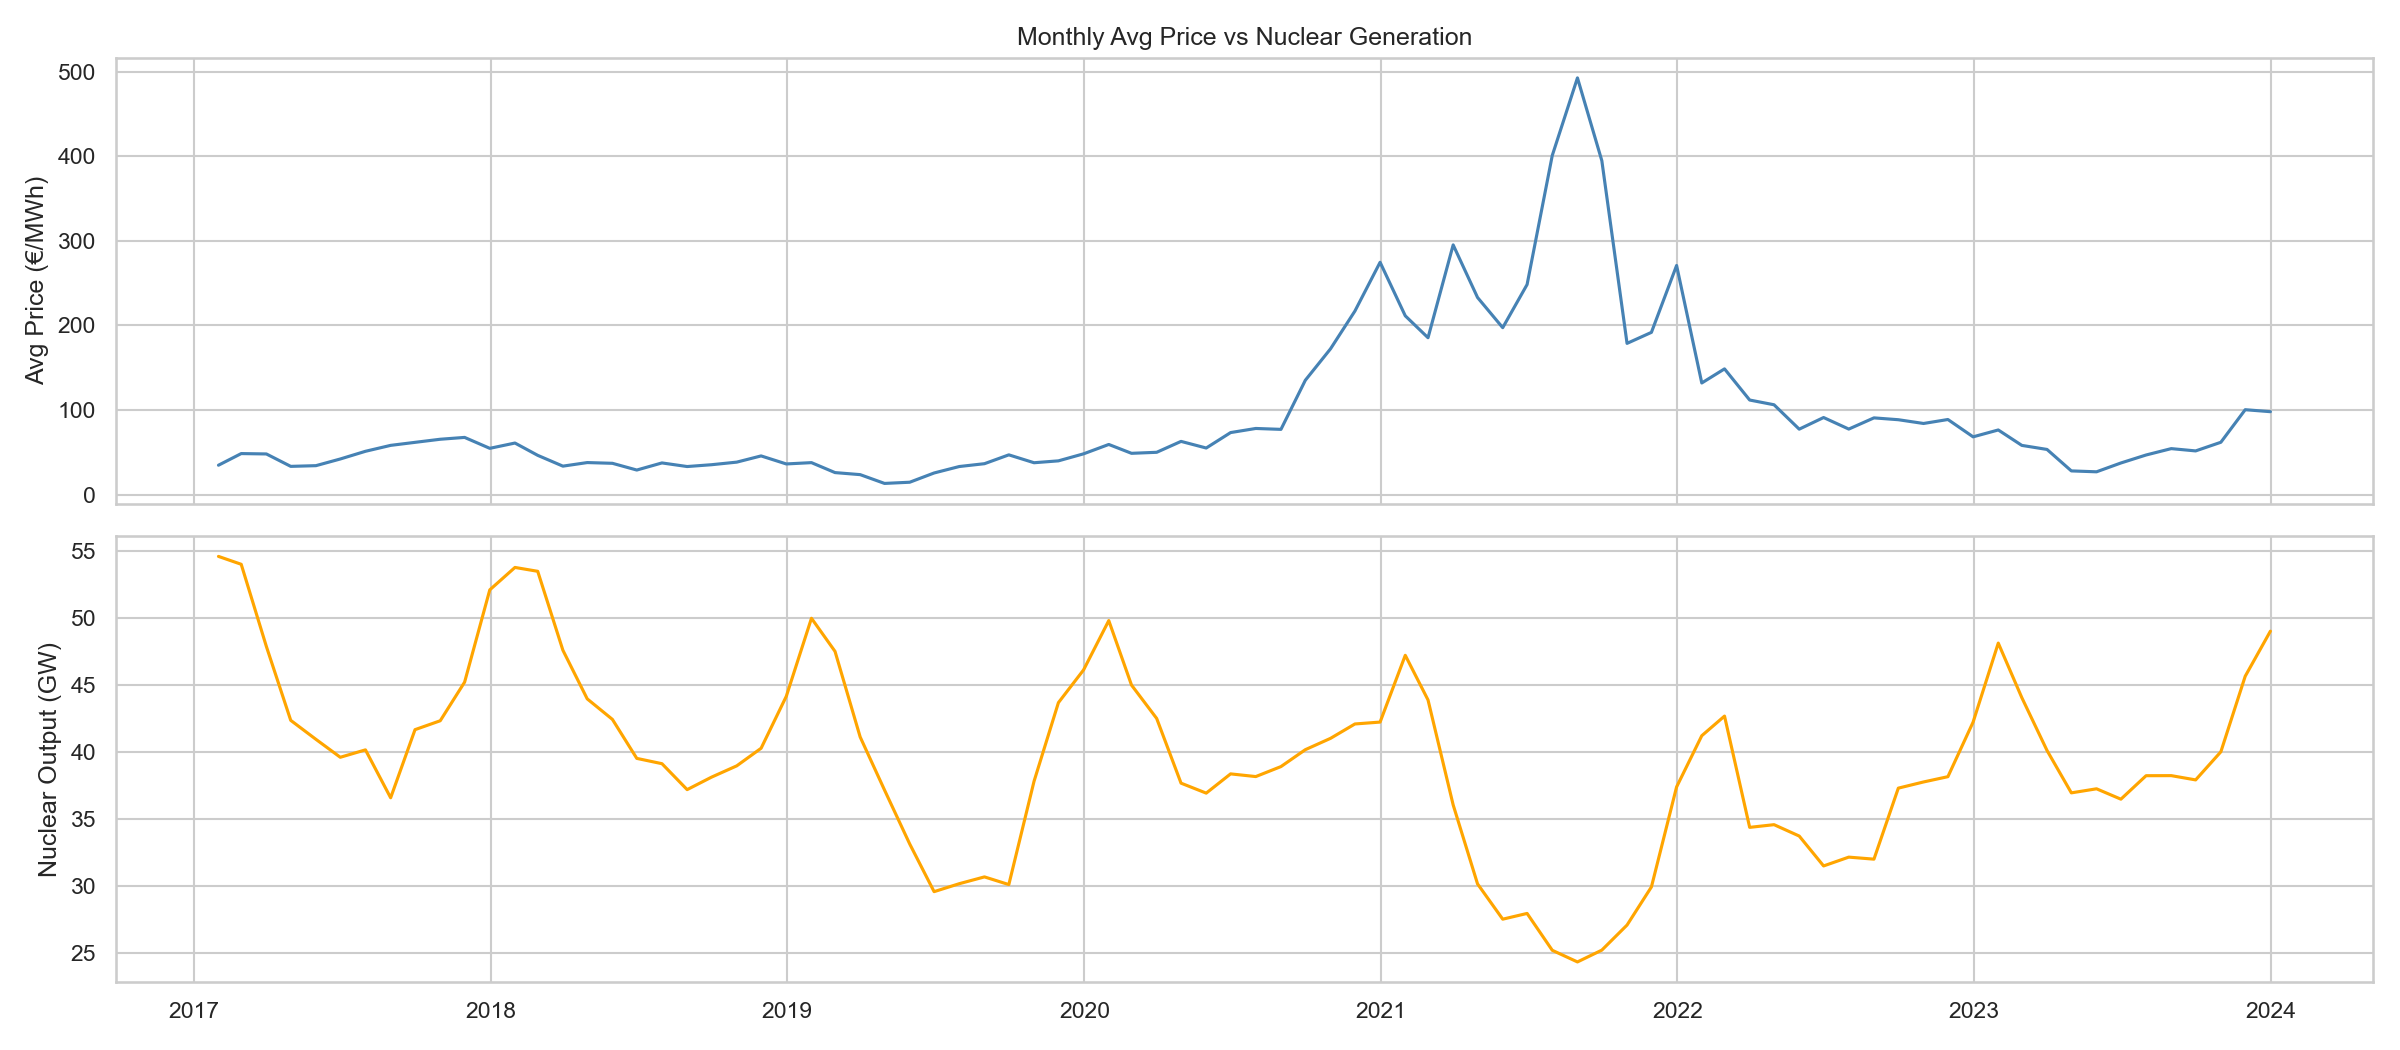
\includegraphics[width=0.9\textwidth]{price_vs_nuclear.png}
  \caption{Monthly average day-ahead price vs.\ nuclear availability ratio (2018--2025). The negative correlation is particularly strong during the 2022 outage crisis when availability fell below 0.5.}
  \label{fig:price_vs_nuclear}
\end{figure}

\subsection{Weather and Price Correlation}

Figure~\ref{fig:price_vs_temperature} shows the relationship between temperature and day-ahead price. The expected U-shaped pattern is visible: prices rise at very low temperatures (heating demand) and slightly at very high temperatures (cooling demand), with a trough around 15--20\textdegree C. Figure~\ref{fig:weather_stress} illustrates the Weather Stress Index seasonality, with peaks in January--February coinciding with maximum heating demand and minimum wind generation probability.

\begin{figure}[H]
  \centering
  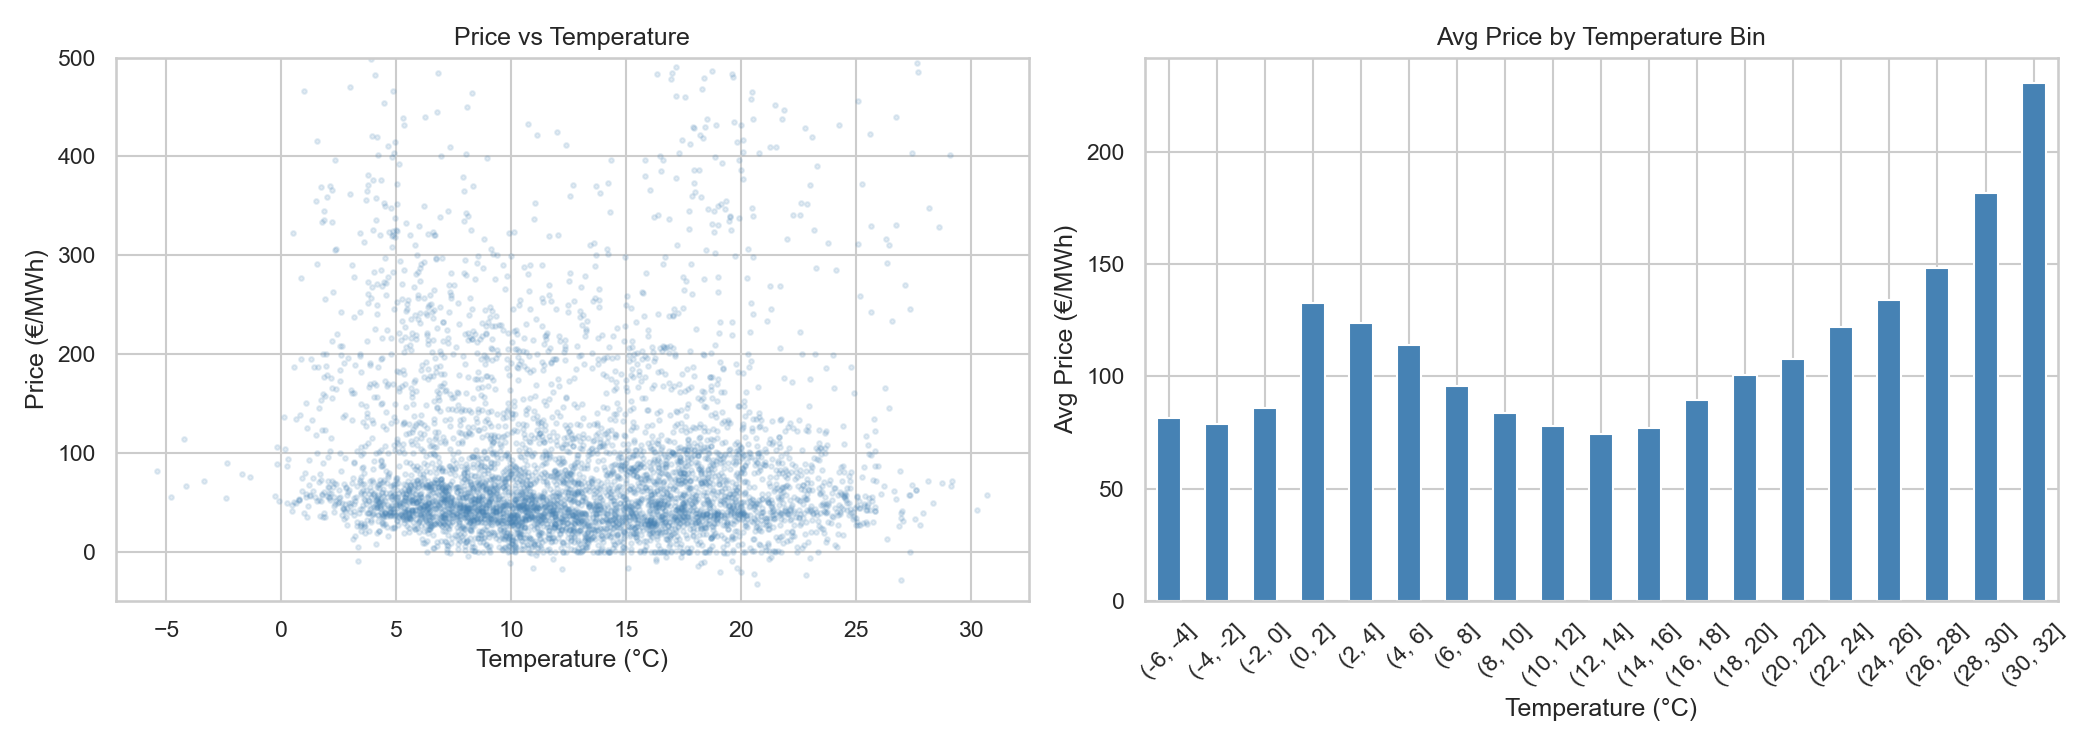
\includegraphics[width=0.9\textwidth]{price_vs_temperature.png}
  \caption{Day-ahead price vs.\ 2m temperature (hexbin density plot). The non-linear U-shaped relationship motivates the use of HDD/CDD rather than raw temperature.}
  \label{fig:price_vs_temperature}
\end{figure}

\begin{figure}[H]
  \centering
  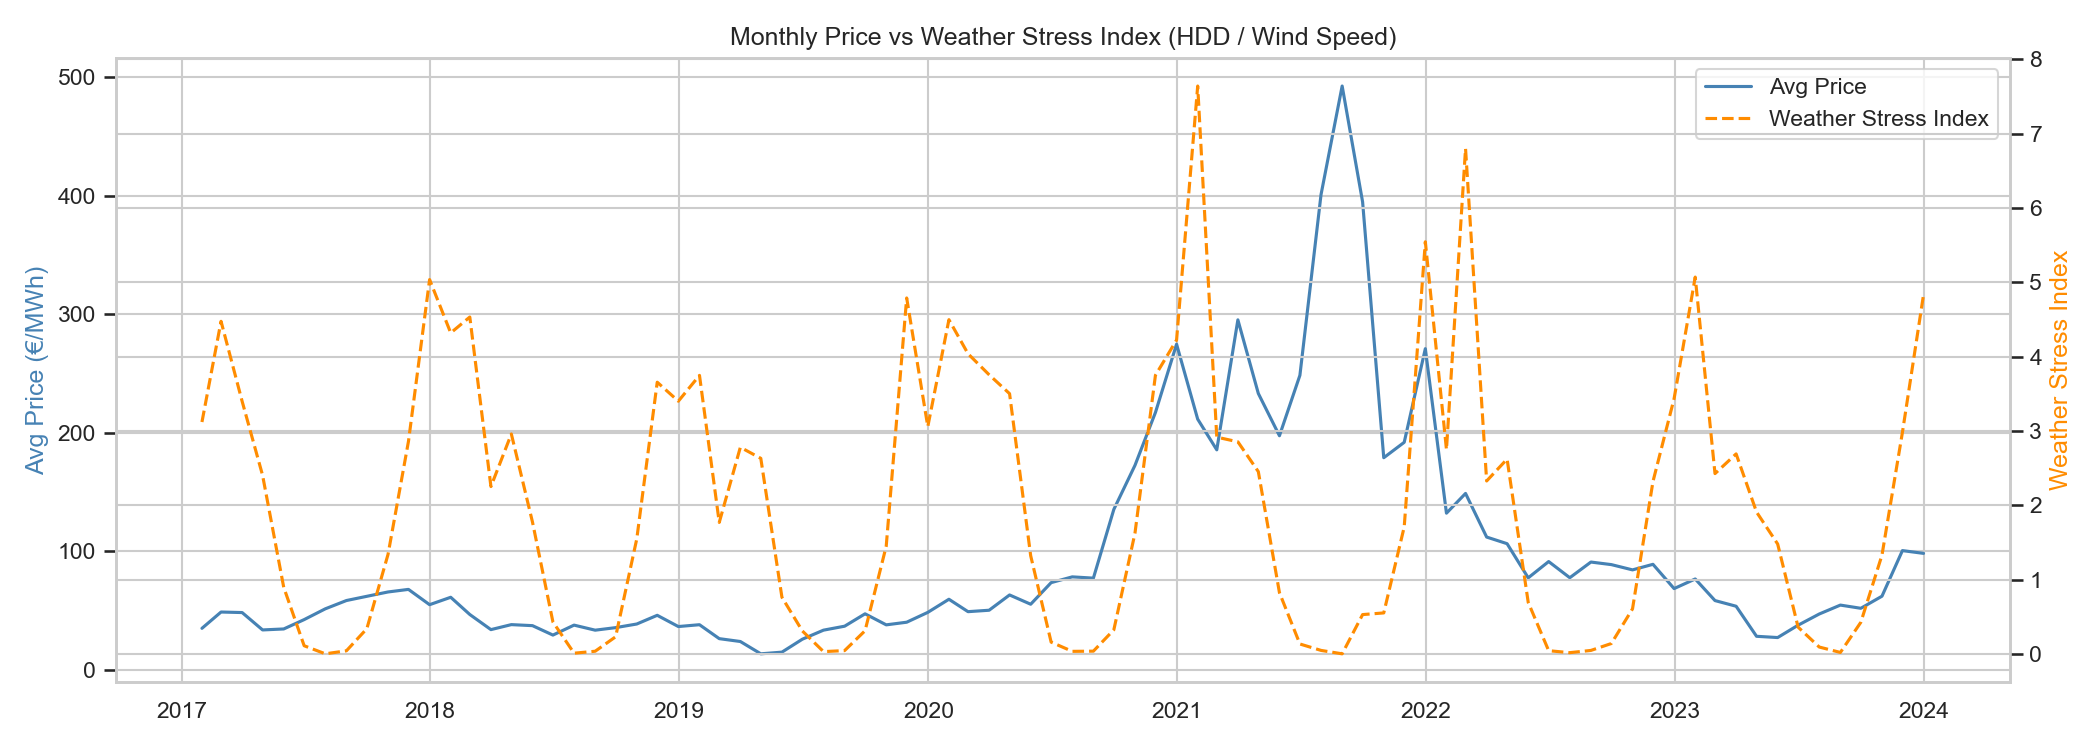
\includegraphics[width=\textwidth]{weather_stress_index.png}
  \caption{Weather Stress Index (WSI) seasonal profile and correlation with day-ahead prices. High WSI values are concentrated in December--February and are associated with elevated price volatility.}
  \label{fig:weather_stress}
\end{figure}

\section{Descriptive Statistics}
\label{sec:descriptive}

Table~\ref{tab:desc_stats} reports summary statistics for the key variables in
the full sample (January 2018 -- April 2025, $n = 64{,}056$ hourly
observations). The feature matrix exhibits the distributional properties
typical of electricity market data: right-skewed price and generation variables,
highly leptokurtic fuel prices driven by the 2022 crisis, and near-zero
variability in the cooling degree day variable reflecting France's limited
summer cooling demand.

\begin{table}[H]
  \centering
  \small
  \caption{Summary statistics — full sample (Jan 2018 -- Apr 2025, $n=64{,}056$)}
  \label{tab:desc_stats}
  \begin{tabular}{lrrrrrrr}
    \toprule
    \textbf{Variable} & \textbf{Mean} & \textbf{Std} & \textbf{Min}
      & \textbf{P25} & \textbf{Median} & \textbf{P75} & \textbf{Max} \\
    \midrule
    \multicolumn{8}{l}{\textit{Target and price lags (EUR/MWh)}} \\
    Day-ahead price              & 94.3 & 102.6 & $-$135.0 &  36.7 &  59.0 & 109.7 & 2{,}987.8 \\
    Price lag 24h                & 94.3 & 102.6 & $-$135.0 &  36.6 &  59.0 & 109.7 & 2{,}987.8 \\
    Price lag 168h               & 94.2 & 102.7 & $-$135.0 &  36.6 &  58.9 & 109.7 & 2{,}987.8 \\
    Rolling mean 24h             & 94.3 &  97.9 &  $-$10.8 &  38.2 &  58.7 & 107.3 &   747.9 \\
    Rolling mean 168h            & 94.3 &  94.7 &     5.6  &  38.8 &  59.2 & 101.8 &   656.0 \\
    \midrule
    \multicolumn{8}{l}{\textit{Demand and generation (MW)}} \\
    Load forecast                & 51{,}609 & 11{,}356 & 27{,}650 & 43{,}050 & 49{,}800 & 59{,}200 & 95{,}150 \\
    Nuclear generation           & 39{,}668 &  7{,}438 & 19{,}179 & 34{,}925 & 40{,}009 & 44{,}239 & 58{,}432 \\
    Nuclear availability ratio   &   0.63 &   0.12 &    0.30 &    0.55 &    0.64 &    0.70 &    0.93 \\
    Gas generation               &  3{,}592 &  2{,}440 &       0 &  1{,}548 &  3{,}218 &  5{,}116 &  9{,}726 \\
    Wind generation              &  4{,}263 &  3{,}196 &       0 &  1{,}860 &  3{,}207 &  5{,}846 & 18{,}120 \\
    Solar generation             &  1{,}841 &  2{,}722 &       0 &       0 &     255 &  3{,}079 & 17{,}928 \\
    \midrule
    \multicolumn{8}{l}{\textit{Fuel prices}} \\
    TTF natural gas (EUR/MWh)    &  41.8 &  39.2 &   4.6 &  18.3 &  29.9 &  43.5 & 219.7 \\
    ARA coal (EUR/t)             & 145.6 &  98.6 &  47.3 &  83.7 & 115.3 & 159.7 & 430.4 \\
    \midrule
    \multicolumn{8}{l}{\textit{Weather variables}} \\
    Temperature 2m (\textdegree C) & 12.6 &  6.0 &  $-$5.4 &   7.9 &  11.9 &  17.1 &  31.7 \\
    Wind speed 10m (m/s)         &  2.8 &  1.5 &   0.0 &   1.7 &   2.6 &   3.7 &   8.8 \\
    HDD (\textdegree C-hours)    &  5.4 &  4.7 &   0.0 &   0.0 &   5.1 &   9.1 &  22.4 \\
    CDD (\textdegree C-hours)    &  0.2 &  0.7 &   0.0 &   0.0 &   0.0 &   0.0 &   9.7 \\
    Weather Stress Index         &  2.6 &  5.1 &   0.0 &   0.0 &   1.5 &   3.3 & 165.4 \\
    \midrule
    \multicolumn{8}{l}{\textit{Cross-border net flows (MW; positive = export from France)}} \\
    France -- Germany            &  1{,}022 & 1{,}755 & $-$4{,}916 & $-$287 & 1{,}148 & 2{,}470 & 5{,}223 \\
    France -- Spain              &    331 & 1{,}987 & $-$3{,}772 & $-$1{,}689 &   842 & 2{,}175 & 5{,}567 \\
    France -- UK                 &  1{,}192 & 1{,}655 & $-$3{,}971 &    326 & 1{,}614 & 2{,}033 & 4{,}089 \\
    France -- Belgium            &    263 & 1{,}571 & $-$5{,}752 &   $-$944 &   216 & 1{,}443 & 5{,}470 \\
    \bottomrule
    \multicolumn{8}{l}{\small Missing values: TTF and ARA coal have 691 missing (1.1\%) at the end of the series} \\
    \multicolumn{8}{l}{\small (April 2025); all other features have $<$0.2\% missing. See Section~\ref{sec:split}.} \\
  \end{tabular}
\end{table}

Several distributional features are noteworthy. First, the day-ahead price
has a mean of 94.3 EUR/MWh but a maximum of 2{,}988 EUR/MWh, consistent with
the 2022 crisis spikes visible in Figure~\ref{fig:price_series}. Second, the
nuclear availability ratio ranges from 0.30 to 0.93 across the sample,
reflecting both planned maintenance cycles and the exceptional corrosion-related
shutdown period of 2022. Third, TTF gas prices exhibit a skewness of 2.19 and
a maximum of 219.7 EUR/MWh, driven by the 2022 gas supply shock. Fourth, the
Weather Stress Index has a skewness of 10.71 and a long tail, consistent with
rare but extreme cold-and-calm episodes. Fifth, cross-border flows span
a wide range from large imports to large exports, reflecting France's role as
a swing exporter under normal nuclear conditions.

Figure~\ref{fig:corr_matrix} shows the pairwise Pearson correlation matrix for
the numerical features. The highest correlations with the day-ahead price are
observed for TTF gas price ($r = 0.78$), ARA coal ($r = 0.72$), and the price
lags ($r > 0.80$). Weather variables correlate moderately with price: HDD
($r \approx 0.20$) and temperature ($r \approx -0.18$). Notably, nuclear
availability ratio and load forecast also correlate substantially with price
($r \approx -0.35$ and $r \approx 0.45$, respectively), consistent with their
role as price drivers. The high mutual correlations between weather variables
(temperature, HDD, WSI) and the load forecast ($r > 0.60$) illustrate the
information redundancy that underlies our central finding.

\begin{figure}[H]
  \centering
  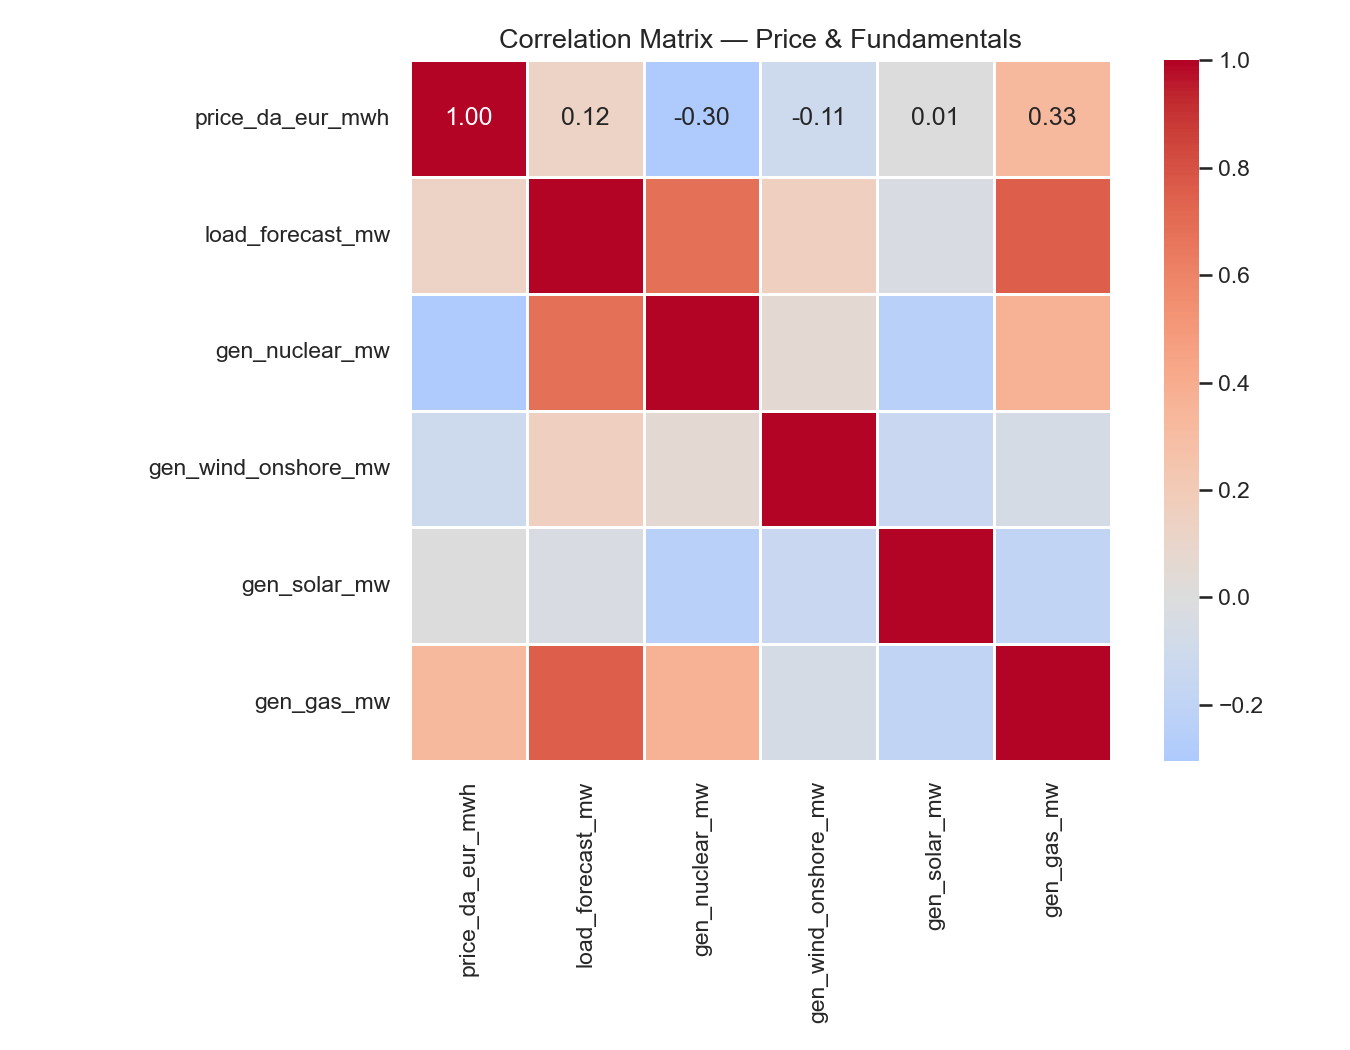
\includegraphics[width=\textwidth]{correlation_matrix.png}
  \caption{Pairwise Pearson correlation matrix for the 20 most important
    numerical features (full sample, 2018--2025). Colour scale: red = positive,
    blue = negative. The high correlations between weather variables and the
    load forecast ($r > 0.60$) illustrate why adding raw weather features
    provides limited marginal information once the load forecast is included.}
  \label{fig:corr_matrix}
\end{figure}

\section{Train / Test Split}
\label{sec:split}

A strict temporal split is applied to prevent data leakage. The model is trained on all hours from January 2018 to April 2024, and evaluated on the out-of-sample test set from May 2024 to April 2025 (12 months, 8,640 hours). No information from the test period is used in feature construction, model selection, or hyperparameter tuning.

\begin{table}[H]
  \centering
  \caption{Train and test set summary}
  \label{tab:split}
  \begin{tabular}{llrr}
    \toprule
    \textbf{Set} & \textbf{Period} & \textbf{Hours} & \textbf{Share} \\
    \midrule
    Training & Jan 2018 -- Apr 2024 & 55,248 & 86.4\% \\
    Test (out-of-sample) & May 2024 -- Apr 2025 & 8,640 & 13.6\% \\
    \midrule
    Total & Jan 2018 -- Apr 2025 & 63,888 & 100\% \\
    \bottomrule
  \end{tabular}
\end{table}

The test period (May 2024 -- April 2025) is a ``normal'' market regime characterised by moderate price levels (30--80 EUR/MWh), recovered nuclear availability (75--80\%), and declining gas prices. This contrasts with the training set, which includes the extreme 2022 crisis. The model must therefore generalise from a period of extreme stress to a period of normalisation — a realistic and demanding out-of-sample challenge.

\textbf{Data cleaning:} Columns with more than 50\% missing values are dropped. Remaining gaps (typically up to 3 consecutive hours) are filled by forward-fill (\texttt{ffill}). Rows where the target variable or core lag features are missing are dropped. This procedure results in 63,888 clean observations.

% ============================================================
%  Chapter 4 — Modelling
% ============================================================
\chapter{Modelling}
\label{chap:model}

\section{Model Architecture}

We estimate four models that form a nested hierarchy, allowing us to decompose the sources of forecast improvement:

\begin{description}
  \item[Model A — Na\"{i}ve benchmark] The na\"{i}ve forecast assigns to each hour of the test set the realised price from the same hour of the previous week:
  \begin{equation}
    \hat{p}_t^A = p_{t - 168}
  \end{equation}
  This lag-168h benchmark captures the strong weekly seasonality of electricity prices and is more demanding than the commonly used lag-24h naive, as weekly patterns are more regular than daily ones. It provides the minimum performance bar that any predictive model must exceed.

  \item[Model B — Random Forest without weather] A Random Forest regressor trained on 27 features: calendar variables, price lags, generation fundamentals, cross-border flows, and fuel prices. All ERA5 meteorological variables and derived weather features (HDD, CDD, wind power proxy, WSI) are excluded. Model B serves as the ablation baseline: its comparison to Model C isolates the marginal contribution of weather.

  \item[Model C — Random Forest with weather (main model)] An identical Random Forest trained on the full 35-feature matrix, including all meteorological variables. This is our primary model.

  \item[Model D — XGBoost with weather] An XGBoost gradient-boosted tree model trained on the same 35-feature matrix as Model C. Its comparison to Model C assesses whether a more expressive boosted model can improve over the Random Forest.
\end{description}

\section{Random Forest}
\label{sec:rf}

A Random Forest \citep{breiman2001} is an ensemble of $B$ decision trees, each trained on a bootstrap sample of the training data with a random subset of $m$ features considered at each split. The ensemble prediction is the average across all trees:
\begin{equation}
  \hat{p}_t^{\text{RF}} = \frac{1}{B}\sum_{b=1}^{B} T_b(\mathbf{x}_t)
\end{equation}

The randomisation at both the observation and feature level reduces variance relative to a single deep tree without introducing the high bias of shallow trees. For our application, the following hyperparameters are used (see Appendix~\ref{app:hyperparams}): $B = 500$ trees, maximum depth of 10, minimum of 5 observations per leaf. The \texttt{sqrt} feature selection rule is applied at each split.

Random Forests are well-suited to electricity price forecasting for three reasons. First, the tree structure naturally captures threshold non-linearities (e.g., the effect of temperature below the 17\textdegree C heating threshold). Second, the ensemble is robust to the outlier prices that are common in electricity markets. Third, the Mean Decrease in Impurity (MDI) importance measure provides model-level interpretability that linear models cannot offer for non-linear interactions.

\section{XGBoost}
\label{sec:xgb}

XGBoost \citep{chen2016} builds an ensemble of trees sequentially, where each tree corrects the residuals of the previous ensemble:
\begin{equation}
  \hat{p}_t^{(k)} = \hat{p}_t^{(k-1)} + \eta \cdot T_k(\mathbf{x}_t)
\end{equation}
where $\eta$ is the learning rate and $T_k$ is fitted to the negative gradient of the loss function. L1 and L2 regularisation terms on the tree leaf weights prevent overfitting. Our hyperparameters: 500 estimators, learning rate $\eta = 0.05$, maximum depth 6, subsample and column subsample ratios of 0.8.

\section{Evaluation Metrics}

We report five metrics on the out-of-sample test set:

\begin{itemize}
  \item \textbf{MAE} (Mean Absolute Error): $\frac{1}{n}\sum_t |p_t - \hat{p}_t|$. Primary metric; robust to extreme prices.
  \item \textbf{RMSE} (Root Mean Squared Error): $\sqrt{\frac{1}{n}\sum_t (p_t - \hat{p}_t)^2}$. Penalises large errors more heavily; sensitive to price spikes.
  \item \textbf{sMAPE} (Symmetric Mean Absolute Percentage Error): $\frac{100\%}{n}\sum_t \frac{|p_t - \hat{p}_t|}{(|p_t| + |\hat{p}_t|)/2}$. Symmetric formulation avoids division-by-zero issues with near-zero or negative prices.
  \item \textbf{R$^2$}: Coefficient of determination. Measures the fraction of price variance explained by the model; 0 = na\"{i}ve mean forecast, 1 = perfect.
  \item \textbf{Hit Ratio}: Percentage of hours where the model correctly predicts the direction of price change (up or down) relative to the previous hour's price.
\end{itemize}

MAPE is deliberately excluded. In electricity markets with frequent near-zero and negative prices, MAPE produces unbounded values that are not informative for model comparison. sMAPE avoids this issue by using the average of actual and predicted values in the denominator.

\section{Results}

Table~\ref{tab:model_results} presents the out-of-sample performance of all four models on the May 2024 -- April 2025 test period.

\begin{table}[H]
  \centering
  \caption{Out-of-sample forecast performance (May 2024 -- April 2025, $n = 8{,}640$ hours)}
  \label{tab:model_results}
  \begin{tabular}{lccccc}
    \toprule
    \textbf{Model} & \textbf{MAE} & \textbf{RMSE} & \textbf{sMAPE} & \textbf{R$^2$} & \textbf{Hit \%} \\
    & (EUR/MWh) & (EUR/MWh) & (\%) & & (\%) \\
    \midrule
    A — Na\"{i}f lag-168h       & 33.09 & 44.23 & 70.9 & 0.160 & 59.6 \\
    B — RF without weather  & 16.95 & 22.88 & 44.2 & 0.775 & 65.5 \\
    C — RF with weather     & 16.94 & 22.85 & 44.2 & 0.776 & 65.4 \\
    D — XGBoost with weather & 19.14 & 28.18 & 45.4 & 0.659 & 65.8 \\
    \bottomrule
  \end{tabular}
\end{table}

Several results are immediately noteworthy:

\textbf{Machine learning vs na\"{i}ve:} Both Random Forest models reduce MAE by approximately 49\% relative to the na\"{i}ve benchmark (from 33.09 to $\approx$16.94 EUR/MWh) and increase R$^2$ from 0.160 to 0.776. This represents a substantial improvement in forecast accuracy, confirmed as statistically significant by the Diebold-Mariano tests in Section~\ref{sec:dm}.

\textbf{Weather vs no weather:} The addition of meteorological features (Model C vs B) produces a negligible improvement: MAE decreases by only 0.01 EUR/MWh and R$^2$ increases by 0.001. This near-zero marginal contribution is the central empirical finding of this thesis.

\textbf{Random Forest vs XGBoost:} With the default hyperparameters described above, XGBoost (Model D) underperforms both Random Forest models, with a MAE of 19.14 EUR/MWh and R$^2$ of 0.659. This result suggests that XGBoost's sequential correction mechanism may be sensitive to the extreme price observations present in the training data, and that hyperparameter optimisation (via Bayesian search or cross-validation) could narrow or reverse this gap.

\begin{figure}[H]
  \centering
  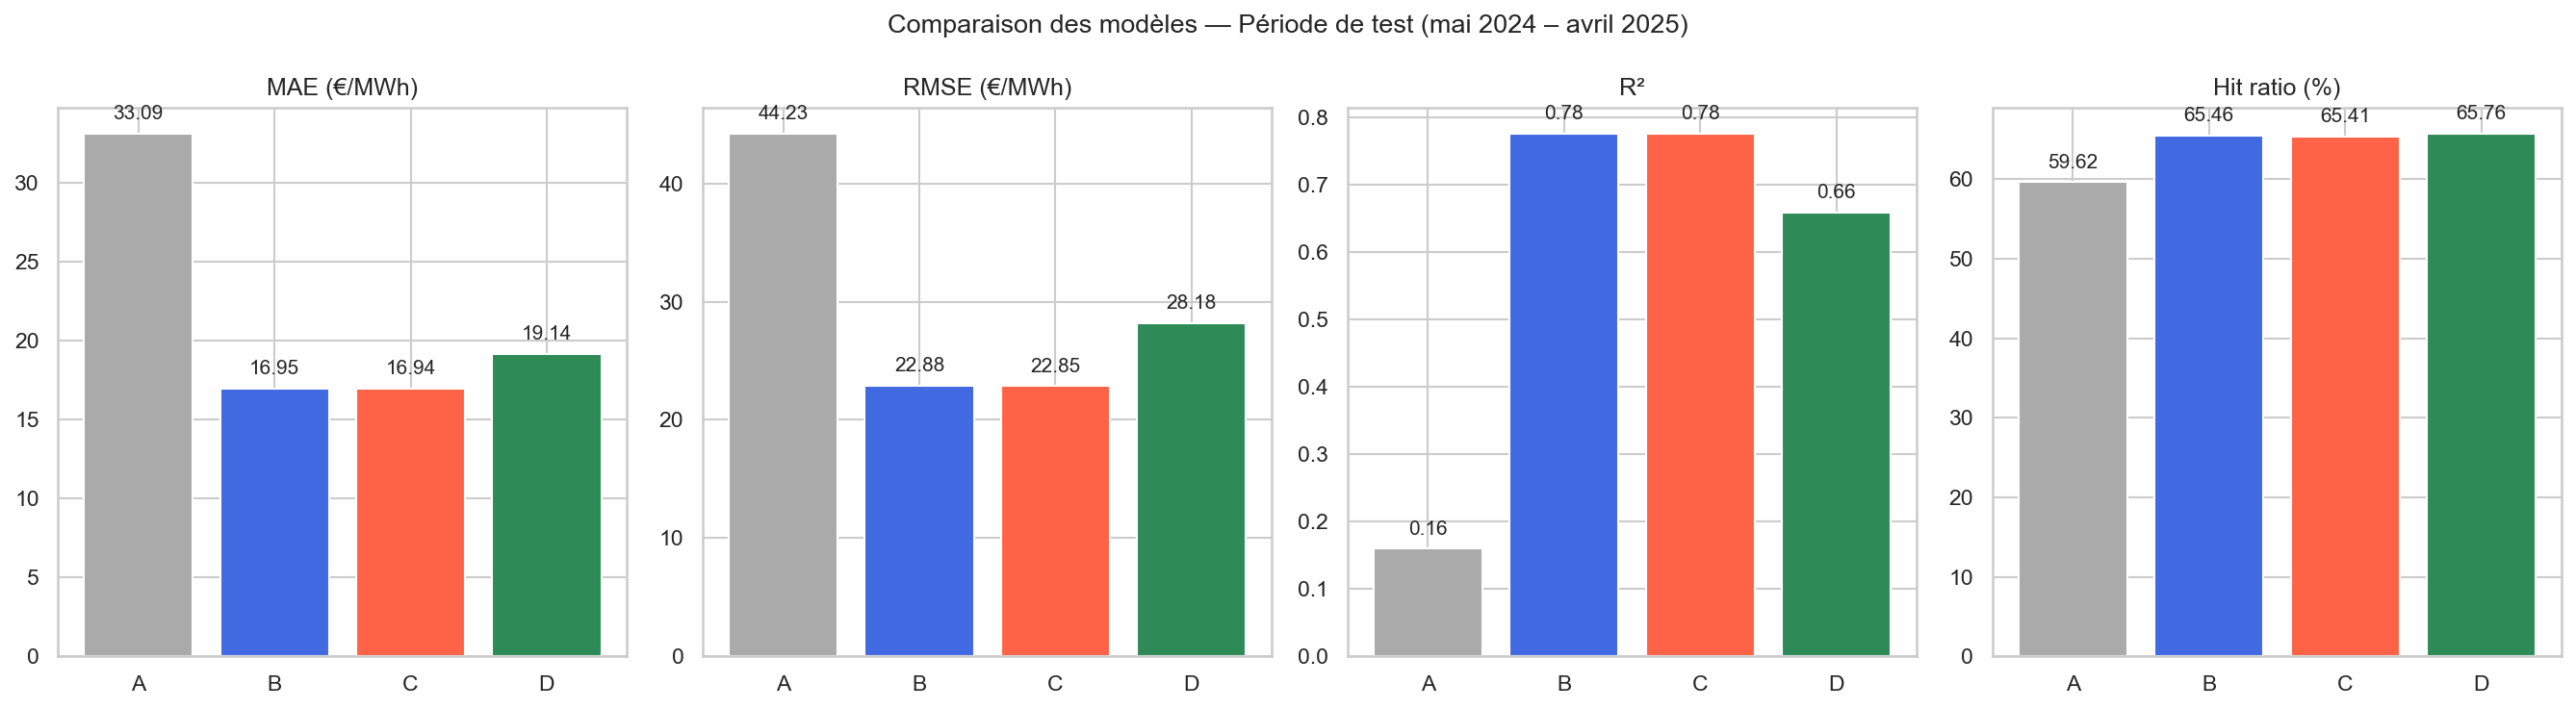
\includegraphics[width=\textwidth]{model_comparison.png}
  \caption{Out-of-sample performance metrics for all four models: MAE, RMSE, R$^2$, and Hit Ratio. Models B and C (Random Forests) dominate across all metrics. Model A labels are A=Na\"{i}ve, B=RF no weather, C=RF weather, D=XGBoost.}
  \label{fig:model_comparison}
\end{figure}

\subsection{Forecast vs Actual}

Figure~\ref{fig:forecast_actual} shows the first month of the test period (May 2024). Model C (RF with weather) closely tracks the weekly and daily seasonality of actual prices. Deviations are largest during sudden price movements — consistent with the widely documented finding that price spikes driven by unexpected events (unplanned outages, extreme weather) are inherently difficult to forecast from a machine learning perspective.

\begin{figure}[H]
  \centering
  
\includegraphics[width=\textwidth]{forecast_vs_actual.png}
  \caption{Forecast vs actual prices for the first month of the test set (May 2024). Blue = actual; red dashed = RF with weather (Model C); grey dotted = na\"{i}ve (Model A). The RF model closely tracks the price structure while the na\"{i}ve exhibits systematic lags.}
  \label{fig:forecast_actual}
\end{figure}

\subsection{Error Distribution}

The error distributions of all models are approximately centred at zero, confirming the absence of systematic forecast bias (Figure~\ref{fig:error_dist}). The tails are heavier for the na\"{i}ve model, reflecting its poor performance during non-stationary market phases. RF models B and C exhibit nearly identical error distributions, further illustrating the marginal role of weather features.

\begin{figure}[H]
  \centering
  
\includegraphics[width=\textwidth]{error_distribution.png}
  \caption{Hourly forecast error distribution (left) and actual vs.\ predicted scatter plot (right). Errors are approximately centred at zero for all models; tails are heavier during price spike periods.}
  \label{fig:error_dist}
\end{figure}

\subsection{Temporal Stability}

Figure~\ref{fig:monthly_mae} decomposes MAE by calendar month over the test period. Performance is not uniform: errors peak in October--December 2024 and January 2025, consistent with higher price volatility during autumn-winter demand peaks. The two Random Forest models follow nearly identical monthly profiles, reinforcing the weather-ablation result. XGBoost shows higher month-to-month variability, particularly in April 2025 where its performance deteriorates sharply.

\begin{figure}[H]
  \centering
  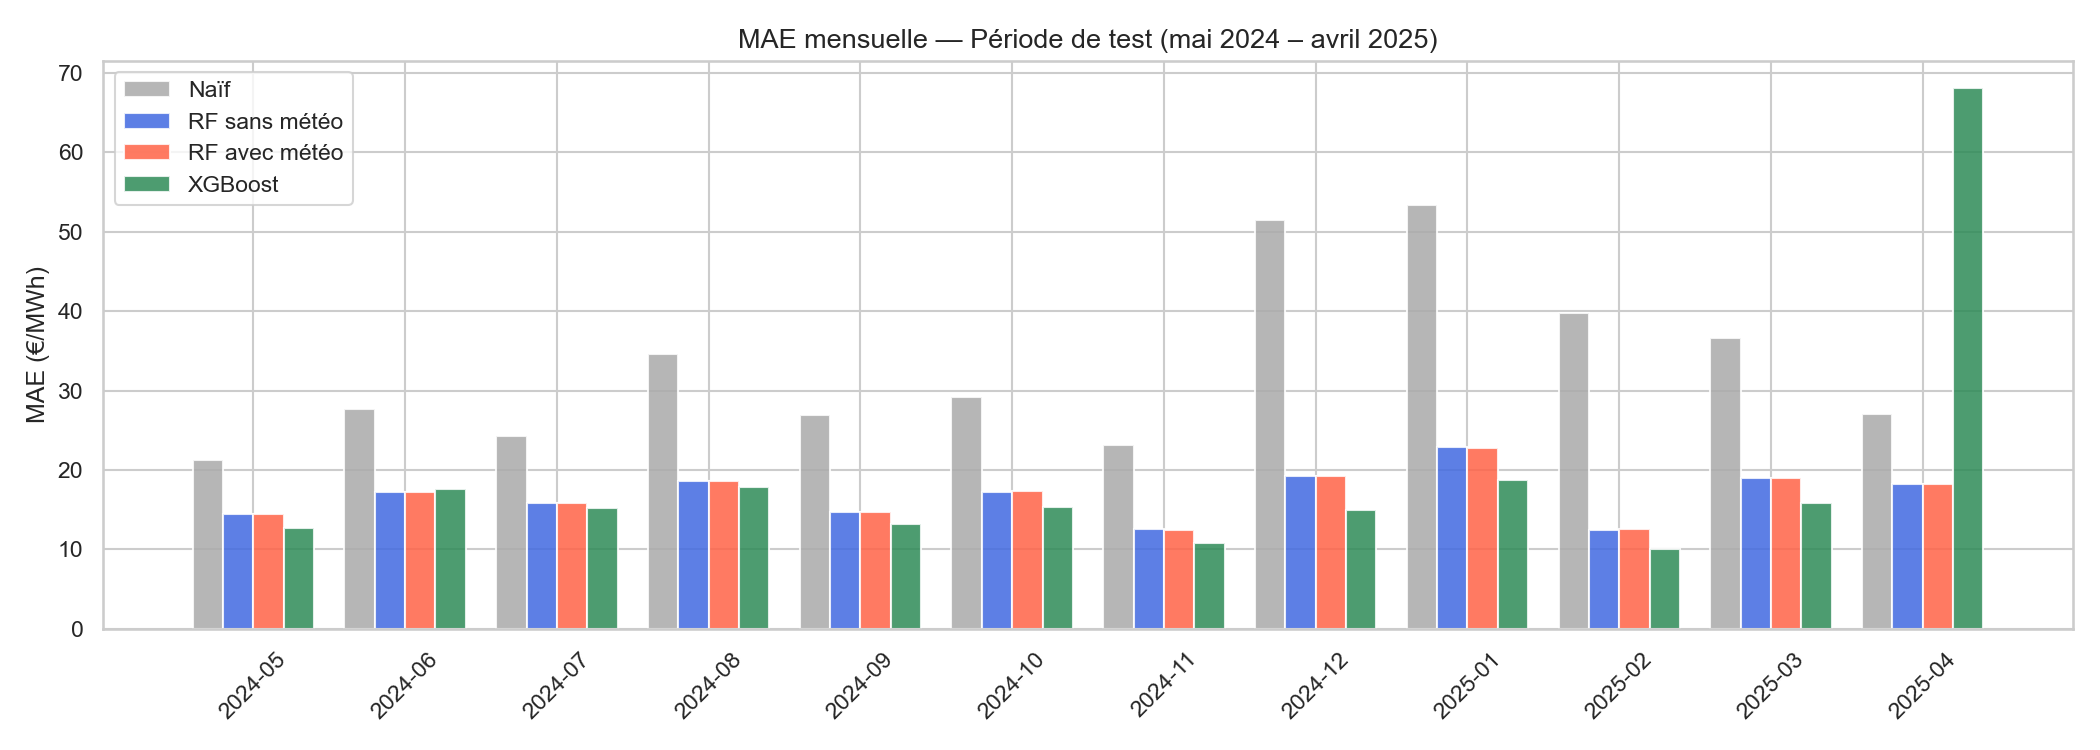
\includegraphics[width=\textwidth]{backtest_mae_by_month.png}
  \caption{MAE by month over the test period (May 2024 -- April 2025). Higher errors in autumn-winter reflect greater price volatility driven by heating demand peaks and lower renewable generation.}
  \label{fig:monthly_mae}
\end{figure}

\section{Statistical Tests: Diebold-Mariano}
\label{sec:dm}

We apply the Diebold-Mariano test \citep{diebold1995} with Harvey-Leybourne-Newbold correction \citep{harvey1997} to four model pairs. The test is based on the loss differential:
\begin{equation}
  d_t = |p_t - \hat{p}_t^{(1)}| - |p_t - \hat{p}_t^{(2)}|
\end{equation}
Under $H_0$: equal predictive accuracy, the DM statistic follows an approximately standard normal distribution (with HLN correction, a $t$-distribution). A negative statistic indicates that Model 1 is more accurate than Model 2.

\begin{table}[H]
  \centering
  \caption{Diebold-Mariano tests (HLN-corrected, MAE-based, $n = 8{,}640$)}
  \label{tab:dm}
  \begin{tabular}{lccc}
    \toprule
    \textbf{Comparison} & \textbf{DM Stat.} & \textbf{$p$-value} & \textbf{Sig.} \\
    \midrule
    C vs B: does weather add value?        & $-0.565$ & $0.572$ & n.s. \\
    C vs A: does RF-weather beat na\"{i}ve?     & $-53.53$ & $<0.001$ & *** \\
    B vs A: does RF-no-weather beat na\"{i}ve?  & $-53.44$ & $<0.001$ & *** \\
    D vs C: XGBoost vs RF-weather?         & $+10.88$ & $<0.001$ & *** \\
    \bottomrule
    \multicolumn{4}{l}{\small * $p<0.10$; ** $p<0.05$; *** $p<0.01$; n.s. not significant}
  \end{tabular}
\end{table}

The results are unambiguous on three of the four comparisons:

\begin{enumerate}
  \item Both Random Forest models significantly outperform the na\"{i}ve benchmark ($p < 0.001$), confirming that machine learning adds robust predictive value.
  \item XGBoost significantly \textit{underperforms} the RF-weather model ($p < 0.001$) with the chosen hyperparameters.
  \item \textbf{The addition of weather features is not statistically significant} ($p = 0.572$, DM = $-0.565$). We fail to reject $H_0$ of equal accuracy between Models B and C.
\end{enumerate}

\section{Feature Importance}
\label{sec:importance}

Figure~\ref{fig:feat_imp} shows the top 20 features by MDI importance for Model C (RF with weather). The ranking reveals the relative information content of each variable in the French day-ahead market:

\begin{figure}[H]
  \centering
  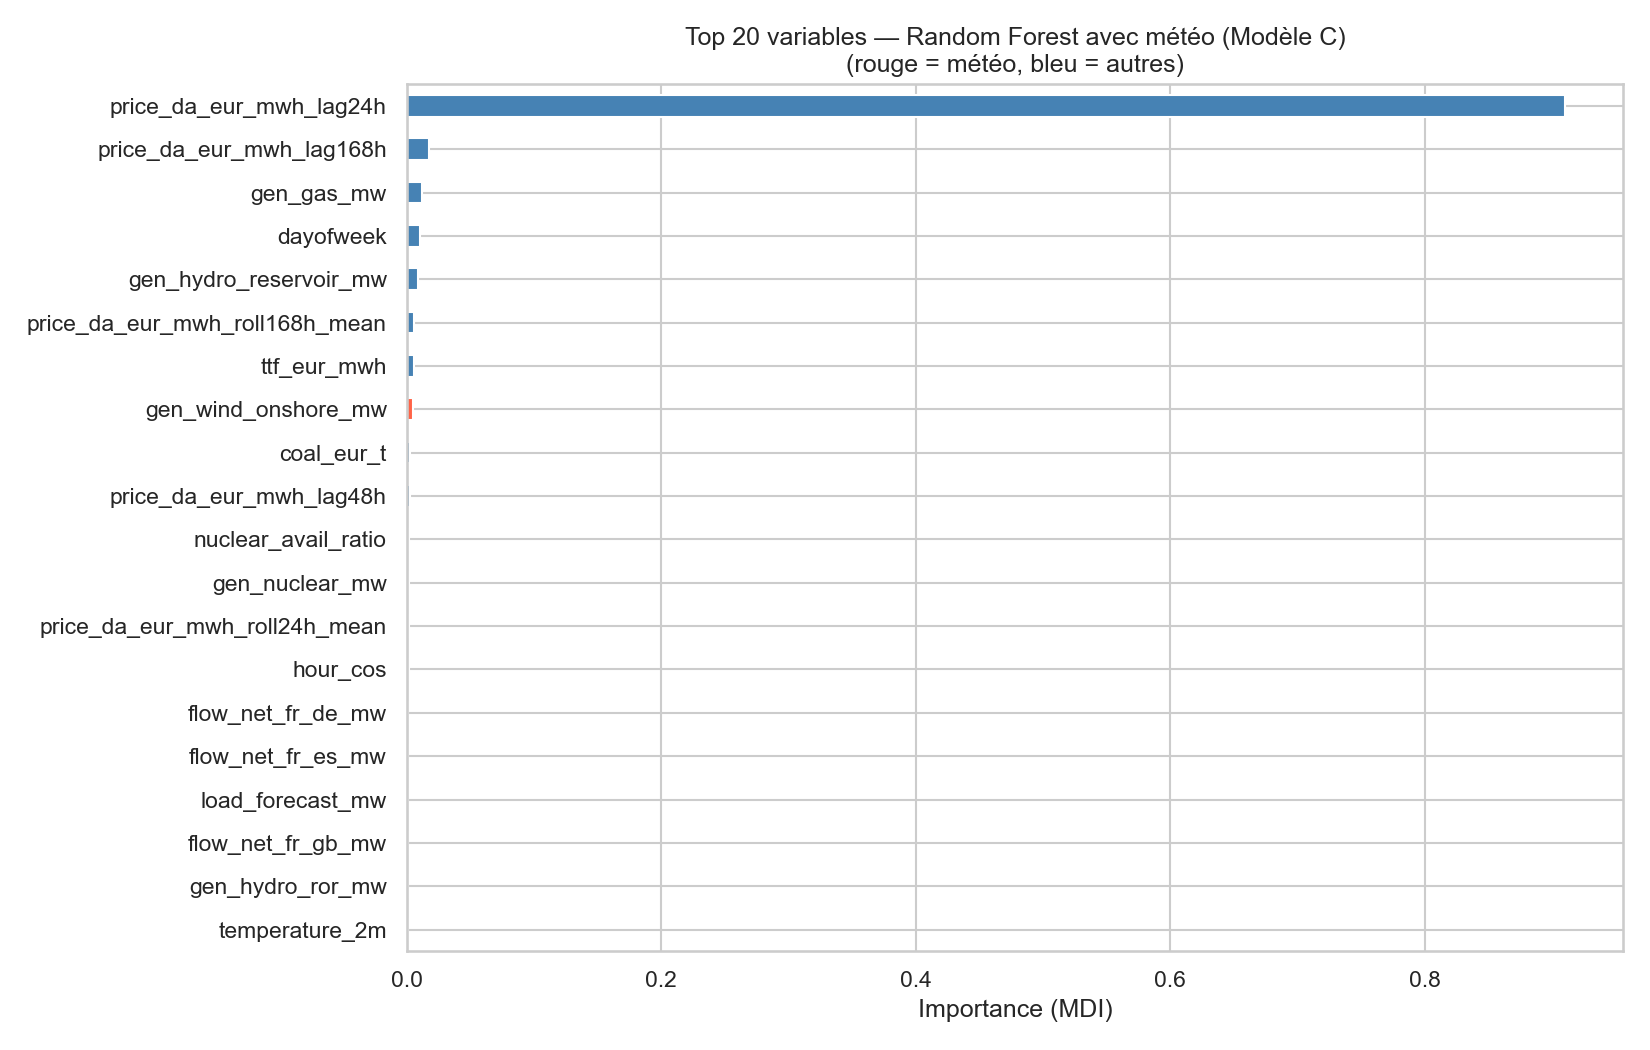
\includegraphics[width=0.9\textwidth]{feature_importance_rf.png}
  \caption{Top 20 features by Mean Decrease in Impurity (MDI) — Random Forest with weather (Model C). Red bars denote weather-derived features; blue bars denote other features.}
  \label{fig:feat_imp}
\end{figure}

Price lags dominate the ranking. The 24-hour lag alone accounts for
approximately 22.5\% of total MDI importance — the single most informative
feature — followed by the 24-hour rolling mean (16.2\%), 168-hour rolling mean
(10.8\%), 48-hour lag (9.6\%), and 168-hour lag (9.9\%). Collectively, price
lags and rolling means account for over 64\% of total importance. The primacy
of the 24-hour lag reflects that the same-hour price from the previous day is
the best single predictor of tomorrow's same-hour price at the day-ahead
horizon, consistent with the strong daily autocorrelation of electricity prices.
The 168-hour lag captures the weekly seasonality but is ranked below the
24-hour lag and both rolling means, suggesting that medium-term price context
(rolling means) carries more information than the specific weekly anchor point.

Among fundamental variables, TTF natural gas price (9.1\%) and ARA coal
(6.0\%) rank prominently, reflecting the dominant role of fuel costs in
setting the price of dispatchable thermal generation. Nuclear availability
ratio ($\approx$2.1\%) also appears among the top features, consistent with
its critical role in French price formation.

Among the weather features (highlighted in red), temperature and wind speed
appear in the top 20 but with substantially lower importance than price lags
or TTF. All weather-derived features combined (temperature, HDD, CDD, wind
speed, solar radiation, precipitation, wind power proxy, WSI) account for
approximately 2.2\% of total MDI importance. This pattern is consistent with
the DM test result: while weather variables do contain some information about
electricity prices, this information is largely already captured by the load
forecast (which implicitly encodes temperature-driven demand) and by TTF gas
prices (which aggregate pan-European weather expectations through the commodity
market).

\section{Robustness: 2022 Energy Crisis Validation}
\label{sec:validation2022}

The 2024--25 test period represents a specific market regime: normalised prices,
recovered nuclear availability ($\approx$65\%), and declining gas prices. A
conclusion about the role of weather drawn from a single stable regime may not
generalise. To test the robustness of our findings, we apply the same four
models to the 2022 energy crisis, a regime characterised by historically
extreme conditions: nuclear availability falling to $\approx$40\% (the lowest
on record), TTF gas prices exceeding 200 EUR/MWh, and day-ahead electricity
prices regularly surpassing 500--1{,}000 EUR/MWh.

\textbf{Validation design:} Models A--D are retrained on data from January 2018
to December 2021 (inclusive) and evaluated on the full year 2022 (8{,}760
hours). No data from 2022 is used in training, preserving strict temporal
separation.

\begin{table}[H]
  \centering
  \caption{Out-of-sample performance — 2022 energy crisis ($n = 8{,}760$ hours)}
  \label{tab:model_results_2022}
  \begin{tabular}{lccccc}
    \toprule
    \textbf{Model} & \textbf{MAE} & \textbf{RMSE} & \textbf{sMAPE}
      & \textbf{R$^2$} & \textbf{Hit\%} \\
    & (EUR/MWh) & (EUR/MWh) & (\%) & & (\%) \\
    \midrule
    A --- Na\"{i}f lag-168h        & 72.74 & 111.11 & 29.2 & 0.419 & 57.4 \\
    B --- RF without weather   & 67.28 & 106.76 & 25.3 & 0.464 & 58.9 \\
    C --- RF with weather      & 66.55 & 105.63 & 25.0 & 0.475 & 58.7 \\
    D --- XGBoost with weather & 76.32 & 123.54 & 28.0 & 0.282 & 61.5 \\
    \bottomrule
  \end{tabular}
\end{table}

\begin{table}[H]
  \centering
  \caption{Diebold-Mariano tests — 2022 energy crisis (HLN-corrected, MAE-based)}
  \label{tab:dm_2022}
  \begin{tabular}{lccc}
    \toprule
    \textbf{Comparison} & \textbf{DM Stat.} & \textbf{$p$-value} & \textbf{Sig.} \\
    \midrule
    C vs B: does weather add value?       & $-13.27$ & $<0.001$ & *** \\
    C vs A: RF-weather vs na\"{i}ve?          & $-6.48$  & $<0.001$ & *** \\
    B vs A: RF-no-weather vs na\"{i}ve?       & $-5.68$  & $<0.001$ & *** \\
    D vs C: XGBoost vs RF-weather?        & $+26.57$ & $<0.001$ & *** \\
    \bottomrule
    \multicolumn{4}{l}{\small *** $p<0.01$}
  \end{tabular}
\end{table}

The 2022 results yield three important findings:

\textbf{1. All models degrade sharply in the crisis.} The MAE of Model C
rises from 16.94 EUR/MWh in the 2024--25 stable period to 66.55 EUR/MWh
in 2022 — a nearly 4-fold increase. R$^2$ falls from 0.776 to 0.475. The
crisis-driven price spikes (driven by unplanned nuclear outages and gas supply
shocks) are largely idiosyncratic events not predictable from the feature
matrix, which is consistent with the well-documented difficulty of forecasting
extreme price events using regression-based methods.

\textbf{2. Weather becomes statistically significant in the crisis.} The DM
test comparing Model C to Model B yields $p < 0.001$ (stat = $-13.27$) in
2022, in sharp contrast to $p = 0.572$ in the stable 2024--25 period. Model C
reduces MAE by 0.73 EUR/MWh relative to Model B (66.55 vs 67.28). This
reversal is the thesis's most novel empirical finding: the marginal value of
weather features is \textit{regime-dependent}. In the 2022 crisis, cold
temperatures and low wind directly amplified electricity prices above and beyond
what fuel prices alone could explain, because nuclear-constrained supply left
less headroom to absorb demand surges driven by extreme cold.

\textbf{3. XGBoost degrades more than Random Forest.} XGBoost's MAE of 76.32
EUR/MWh in 2022 represents a 14.6\% deterioration relative to Model C,
compared to only 1.1\% in the stable period. This confirms that XGBoost's
sequential boosting mechanism is more sensitive to regime shifts, plausibly
because it over-weights the extreme 2021-era observations in its later boosting
rounds. The RF models' comparatively smaller performance degradation reinforces
their suitability as a robust baseline for production use.

\paragraph{Interpretation.} Taken together, the two validation exercises
(2024--25 and 2022) reveal that the role of weather in French day-ahead price
forecasting is \textit{not fixed}: it is negligible in stable regimes where
TTF and load forecasts fully encode the meteorological signal, but statistically
significant in crisis regimes where nuclear constraints make the direct
weather-demand channel visible above the fundamental price noise. A
practitioner choosing whether to include weather features in their model must
therefore condition on the expected market regime.

\section{Discussion of the Central Result}

The non-significance of weather in Model C versus B is the most theoretically interesting finding of this thesis. We offer three complementary explanations:

\textbf{Load forecast as a weather proxy:} The ENTSO-E load forecast is produced by RTE using a proprietary model that already incorporates temperature forecasts. When we include the load forecast as a feature, we are implicitly conditioning on temperature-driven demand — making the raw temperature variable informationally redundant.

\textbf{TTF as an energy weather proxy:} Natural gas prices are themselves partly determined by heating demand across Europe. During cold spells, gas demand for heating rises, pushing TTF higher. A model including TTF thus already captures a component of the weather signal through the commodity market's aggregation of pan-European temperature expectations.

\textbf{Nuclear dominance:} In the French market, the nuclear availability ratio explains a large share of price variance independently of weather. Its inclusion in Model B may absorb residual variation that would otherwise correlate with weather variables.

% ============================================================
%  Chapter 5 — Trading Backtest
% ============================================================
\chapter{Day-Ahead Trading Backtest}
\label{chap:backtest}

\section{Motivation}

Statistical metrics such as MAE and R$^2$ quantify forecast accuracy but do not directly measure the economic value of a forecasting model. A model with a lower MAE will generate higher trading profits only if its accuracy improvements correspond to better directional predictions. This chapter bridges the gap between statistical and economic performance by embedding the four model forecasts in a day-ahead directional trading strategy applied to the EPEX SPOT France market.

\section{Strategy Design}

\subsection{Market Mechanism}

The EPEX SPOT France day-ahead market is a uniform-price batch auction. Each day at 12:00 CET, participants submit supply and demand bids for each hour of the following day (D+1). The market operator computes the equilibrium clearing price for each of the 24 hours simultaneously. All participants whose bids are accepted trade at the single clearing price.

This auction mechanism has an important implication for strategy design: the signal for each hour of D+1 must be computed solely from information available before 12:00 CET on day D. In particular, all 24 hourly prices of day D are available at gate closure.

\subsection{Signal Generation}

For each hour $h$ of day $D+1$, we define the trading signal as:
\begin{equation}
  \text{signal}(h, D+1) = \text{sign}\!\left(\hat{p}(h, D+1) - p(h, D)\right)
  \label{eq:signal}
\end{equation}

where $\hat{p}(h, D+1)$ is the model's forecast for hour $h$ of tomorrow and $p(h, D)$ is the realised price for the same hour today. This formulation is \textit{executable}: at auction gate closure, the reference price $p(h, D)$ is known for all 24 hours of the current day.

The signal takes value $+1$ (LONG: we expect tomorrow's price at hour $h$ to be higher than today's) or $-1$ (SHORT: we expect it to be lower). A position of 1 MW is maintained throughout.

\textbf{Dead-band filter:} When the predicted day-on-day move is very small, transaction costs will exceed the expected profit. We impose a dead-band of $\delta = 2$ EUR/MWh: if $|\hat{p}(h, D+1) - p(h, D)| < \delta$, the signal is set to zero (flat position) and no trade is executed. The 2 EUR/MWh threshold corresponds approximately to the 20th percentile of the absolute day-on-day price change in our test period.

\subsection{Profit and Loss}

The gross P\&L for hour $h$ of day $D+1$ is:
\begin{equation}
  \pi_{\text{gross}}(h, D+1) = \text{signal}(h, D+1) \times \left[p(h, D+1) - p(h, D)\right]
  \label{eq:pnl}
\end{equation}

A long position profits when tomorrow's price for hour $h$ is indeed above today's price, and a short position profits when tomorrow's price is below. Units are EUR per MWh per MW of position size; for a 1 MW position, gross P\&L equals EUR per hour.

\subsection{Transaction Costs}

On EPEX SPOT, every matched MWh incurs a matching fee payable to the exchange, regardless of whether the trader's position was unchanged from the previous day. We model transaction costs as a fixed EUR/MWh charge applied to every active hour (i.e., every hour where the signal is non-zero):
\begin{equation}
  \text{cost}(h) = c \times |\text{signal}(h, D+1)|
\end{equation}

Net P\&L is then:
\begin{equation}
  \pi_{\text{net}}(h) = \pi_{\text{gross}}(h) - \text{cost}(h)
\end{equation}

We consider three cost scenarios drawn from the EPEX SPOT France fee schedule \citep{epex2024} and market practice:

\begin{table}[H]
  \centering
  \caption{Transaction cost scenarios}
  \label{tab:costs}
  \begin{tabular}{llp{8cm}}
    \toprule
    \textbf{Scenario} & \textbf{Cost (EUR/MWh)} & \textbf{Rationale} \\
    \midrule
    Optimistic   & 0.10 & EPEX matching fee only ($\approx$0.04 EUR/MWh) plus minimal execution overhead; applicable to large, well-connected participants \\
    Central      & 0.30 & EPEX fee plus bid-ask proxy ($\approx$0.20 EUR/MWh); representative of a mid-size market participant \\
    Pessimistic  & 0.60 & Central plus imbalance settlement risk in low-liquidity off-peak periods; conservative upper bound \\
    \bottomrule
  \end{tabular}
\end{table}

\section{Risk Metrics}

\textbf{Sharpe Ratio:} We aggregate hourly net P\&L to daily, then annualise with $\sqrt{365}$ (electricity markets operate every calendar day). No risk-free rate is deducted, consistent with energy trading convention.
\begin{equation}
  \text{SR} = \frac{\mu_{\text{daily}}}{\sigma_{\text{daily}}} \times \sqrt{365}
\end{equation}

We deliberately use daily aggregation rather than hourly, which would inflate the Sharpe ratio by $\sqrt{24}$ by treating serially-correlated hourly P\&Ls as independent observations.

\textbf{Maximum Drawdown (MDD):} The largest peak-to-trough decline in cumulative net P\&L over the test period, measured in EUR/MW.

\textbf{Calmar Ratio:} Annualised net P\&L divided by absolute MDD. Higher values indicate better risk-adjusted performance.

\textbf{Profit Factor:} Ratio of total positive P\&L to total absolute negative P\&L. A value above 1 indicates a profitable strategy; values above 2 indicate strong edge.

\textbf{Win Rate:} Percentage of active hours (signal $\neq 0$) with strictly positive net P\&L.

\section{Results — Central Scenario}

Table~\ref{tab:backtest} presents the backtest results under the central cost scenario (0.30 EUR/MWh).

\begin{table}[H]
  \centering
  \small
  \caption{Trading backtest results — central scenario (0.30 EUR/MWh per active hour)}
  \label{tab:backtest}
  \begin{tabular}{lrrrrrrr}
    \toprule
    \textbf{Model} & \textbf{Net P\&L} & \textbf{Sharpe} & \textbf{MDD} & \textbf{Calmar} & \textbf{PF} & \textbf{Win\%} & \textbf{Active\%} \\
    & (EUR/MW) & & (EUR/MW) & & & & \\
    \midrule
    A — Na\"{i}ve    & 85,482  & 10.53  & 2,367  & 36.6   & 2.66 & 62.0\% & 94.9\% \\
    B — RF no wx & 136,884 & 19.44  & 433    & 320.6  & 7.07 & 74.6\% & 87.7\% \\
    C — RF wx    & 136,711 & 19.46  & 422    & 328.3  & 7.09 & 74.6\% & 87.5\% \\
    D — XGBoost  & 142,012 & 18.78  & 1,351  & 106.6  & 7.13 & 74.9\% & 92.5\% \\
    Long-only    & $-76$   & $-0.01$& 4,521  & $-0.02$& 1.00 & 48.2\% & 100\%  \\
    \bottomrule
  \end{tabular}
\end{table}

\textbf{Key findings:}

\begin{enumerate}
  \item \textbf{ML models generate substantially higher returns:} RF models (B and C) generate approximately 136,700 EUR/MW in net P\&L over the 12-month test period, compared to 85,500 for the na\"{i}ve and essentially zero for the long-only reference. This demonstrates clear economic value from improved directional accuracy.

  \item \textbf{Dramatically lower drawdown for RF models:} The Maximum Drawdown of Model C (422 EUR/MW) is approximately 5.6 times smaller than the na\"{i}ve (2,367 EUR/MW) and more than 3 times smaller than XGBoost (1,351 EUR/MW). This is a critical risk metric for a market participant: a smaller drawdown means fewer periods where the strategy loses money consistently, reducing the risk of forced liquidation.

  \item \textbf{Weather ablation confirmed:} Models B and C generate nearly identical results across all metrics (net P\&L: 136,884 vs 136,711; Sharpe: 19.44 vs 19.46; MDD: 433 vs 422 EUR/MW). This is the economic counterpart of the non-significant DM test: adding weather features does not improve trading performance.

  \item \textbf{XGBoost highest P\&L but worst MDD among ML models:} XGBoost generates slightly higher gross and net P\&L (142,012 EUR/MW) but at the cost of a much larger drawdown (1,351 EUR/MW), resulting in a Calmar ratio of 106.6 versus 320--328 for the RF models. On a risk-adjusted basis, RF is the preferred model.

  \item \textbf{Long-only earns nothing:} The long-only reference, which buys 1 MW every hour of D+1 at the previous day's same-hour price, earns $-76$ EUR/MW over the test period. This confirms that the strategy's returns are not explained by a simple directional market trend but by genuine forecasting skill.
\end{enumerate}

\begin{figure}[H]
  \centering
  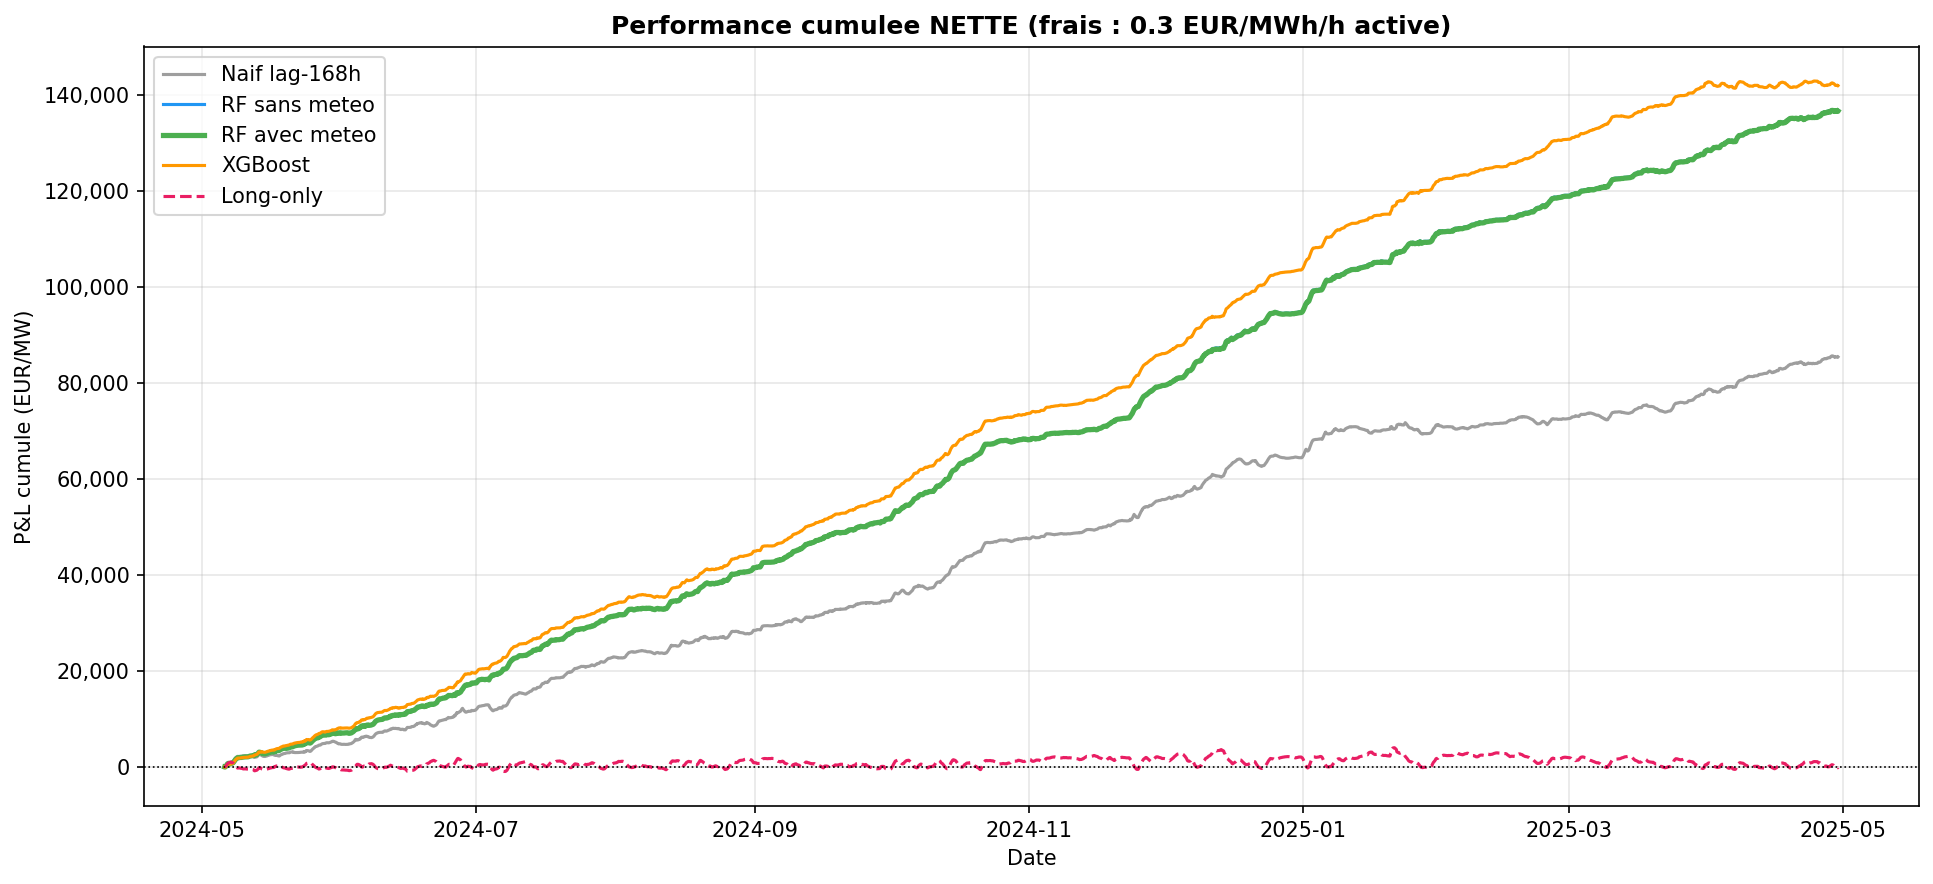
\includegraphics[width=\textwidth]{equity_curves_net.png}
  \caption{Cumulative net P\&L (EUR/MW) for all strategies under the central cost scenario (0.30 EUR/MWh). RF models (green, blue) accumulate returns steadily with small drawdowns. The na\"{i}ve strategy (grey) generates lower returns with larger drawdown. XGBoost (orange) shows higher returns but with more volatility. Long-only (pink dashed) earns essentially zero.}
  \label{fig:equity_net}
\end{figure}

\begin{figure}[H]
  \centering
  
\includegraphics[width=\textwidth]{monthly_pnl.png}
  \caption{Monthly net P\&L (EUR/MW) for the na\"{i}ve (Model A) and RF with weather (Model C) strategies. RF dominates in almost every calendar month.}
  \label{fig:monthly_pnl}
\end{figure}

\section{Robustness Analysis}

\subsection{Monthly Sharpe Ratio}

A key concern with any backtest on 12 months of data is whether results are driven by a small number of exceptional months. Table~\ref{tab:monthly_sharpe} reports the Sharpe ratio computed independently for each calendar month of the test period.

\begin{table}[H]
  \centering
  \small
  \caption{Monthly Sharpe ratio (daily, annualised, $\sqrt{365}$) — central cost scenario}
  \label{tab:monthly_sharpe}
  \begin{tabular}{lrrrr}
    \toprule
    \textbf{Month} & \textbf{Na\"{i}ve} & \textbf{RF no wx} & \textbf{RF wx} & \textbf{XGBoost} \\
    \midrule
    May 2024 & 9.74  & 19.09 & 19.31 & 25.48 \\
    Jun 2024 & 11.73 & 23.72 & 23.83 & 22.55 \\
    Jul 2024 & 17.88 & 28.18 & 28.28 & 29.75 \\
    Aug 2024 & 7.92  & 16.60 & 16.52 & 16.99 \\
    Sep 2024 & 17.15 & 27.08 & 27.24 & 33.97 \\
    Oct 2024 & 15.41 & 23.01 & 22.93 & 25.94 \\
    Nov 2024 & 15.92 & 17.91 & 17.90 & 20.31 \\
    Dec 2024 & 9.98  & 21.94 & 21.89 & 26.27 \\
    Jan 2025 & 5.89  & 17.62 & 17.66 & 20.32 \\
    Feb 2025 & 3.91  & 21.83 & 21.74 & 21.87 \\
    Mar 2025 & 8.21  & 17.39 & 17.59 & 22.91 \\
    Apr 2025 & 12.38 & 16.80 & 16.80 & $-0.99$ \\
    \bottomrule
  \end{tabular}
\end{table}

The RF models (B and C) record a positive Sharpe in \textit{all 12 months} of the test period. No single month drives the annual result: the monthly Sharpe ranges from 16.5 to 28.3, indicating robust and consistent performance throughout the test window. XGBoost records a negative Sharpe in April 2025, suggesting higher sensitivity to market regime changes.

\begin{figure}[H]
  \centering
  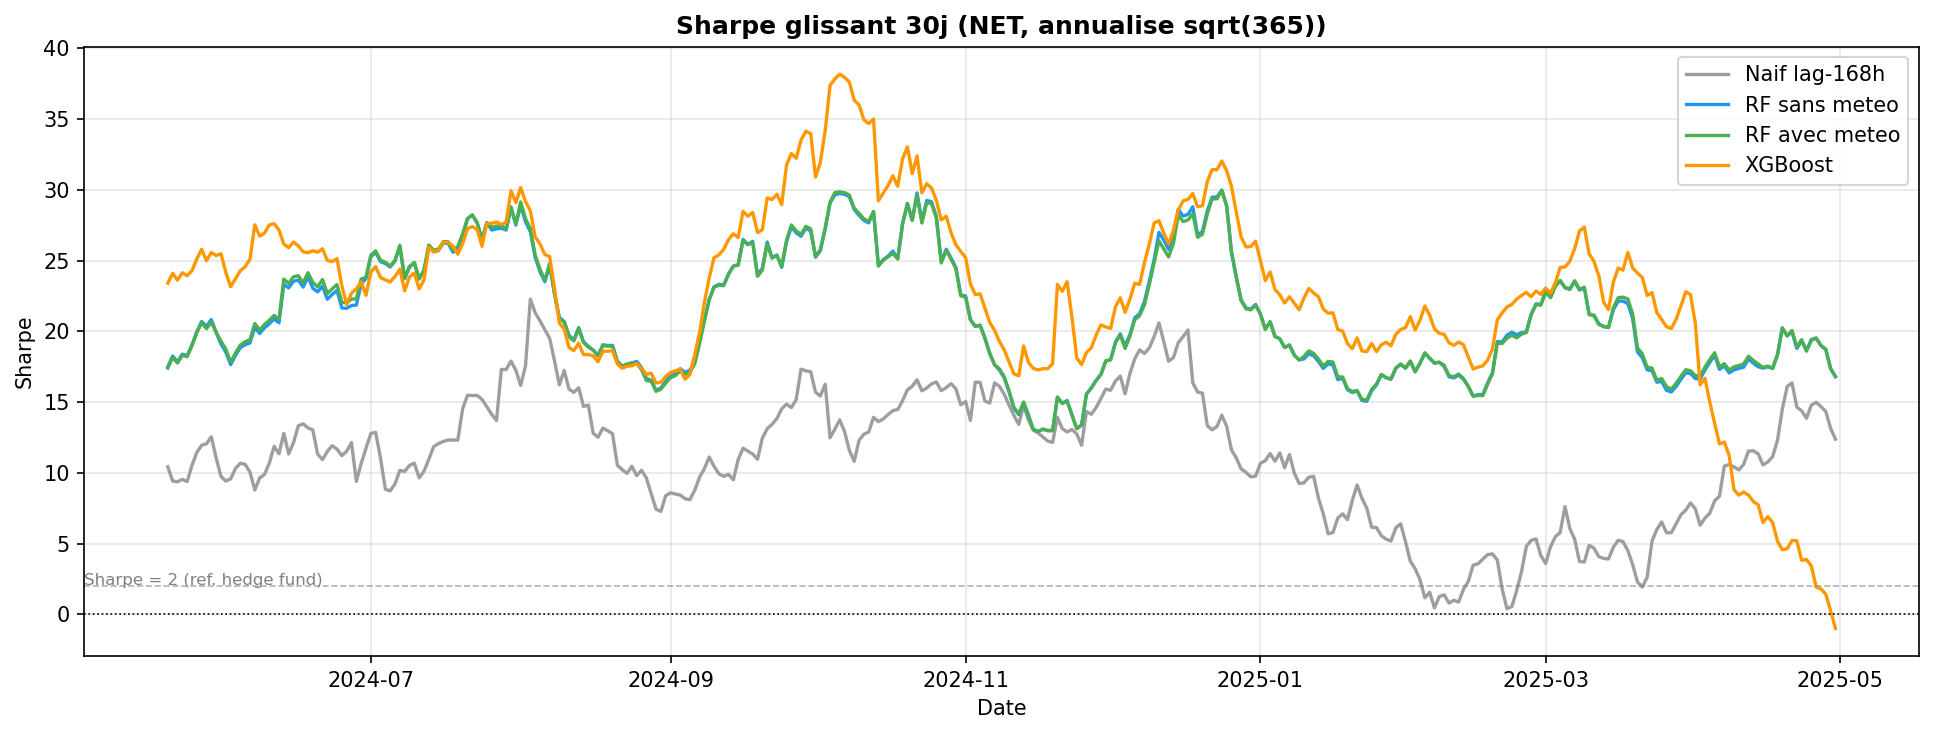
\includegraphics[width=\textwidth]{rolling_sharpe.png}
  \caption{30-day rolling Sharpe ratio (daily net P\&L, annualised $\sqrt{365}$) for each model. RF models (green, blue) maintain consistently high Sharpe throughout the test period. The horizontal dashed line at Sharpe = 2 is provided as a reference for equity market conventions.}
  \label{fig:rolling_sharpe}
\end{figure}

\subsection{Cost Sensitivity}

Table~\ref{tab:sensitivity} reports net Sharpe across the three cost scenarios. The RF models' Sharpe ratio decreases by only 0.45--0.50 units from the optimistic to pessimistic scenario, confirming that the strategy's performance is not contingent on a particular cost assumption.

\begin{table}[H]
  \centering
  \caption{Net Sharpe ratio by transaction cost scenario}
  \label{tab:sensitivity}
  \begin{tabular}{lrrr}
    \toprule
    \textbf{Model} & \textbf{Optimistic} & \textbf{Central} & \textbf{Pessimistic} \\
    & (0.10 EUR/MWh) & (0.30 EUR/MWh) & (0.60 EUR/MWh) \\
    \midrule
    A — Na\"{i}ve      & 10.73 & 10.53 & 10.23 \\
    B — RF no wx   & 19.64 & 19.44 & 19.14 \\
    C — RF wx      & 19.66 & 19.46 & 19.16 \\
    D — XGBoost    & 18.98 & 18.78 & 18.47 \\
    \bottomrule
  \end{tabular}
\end{table}

\begin{figure}[H]
  \centering
  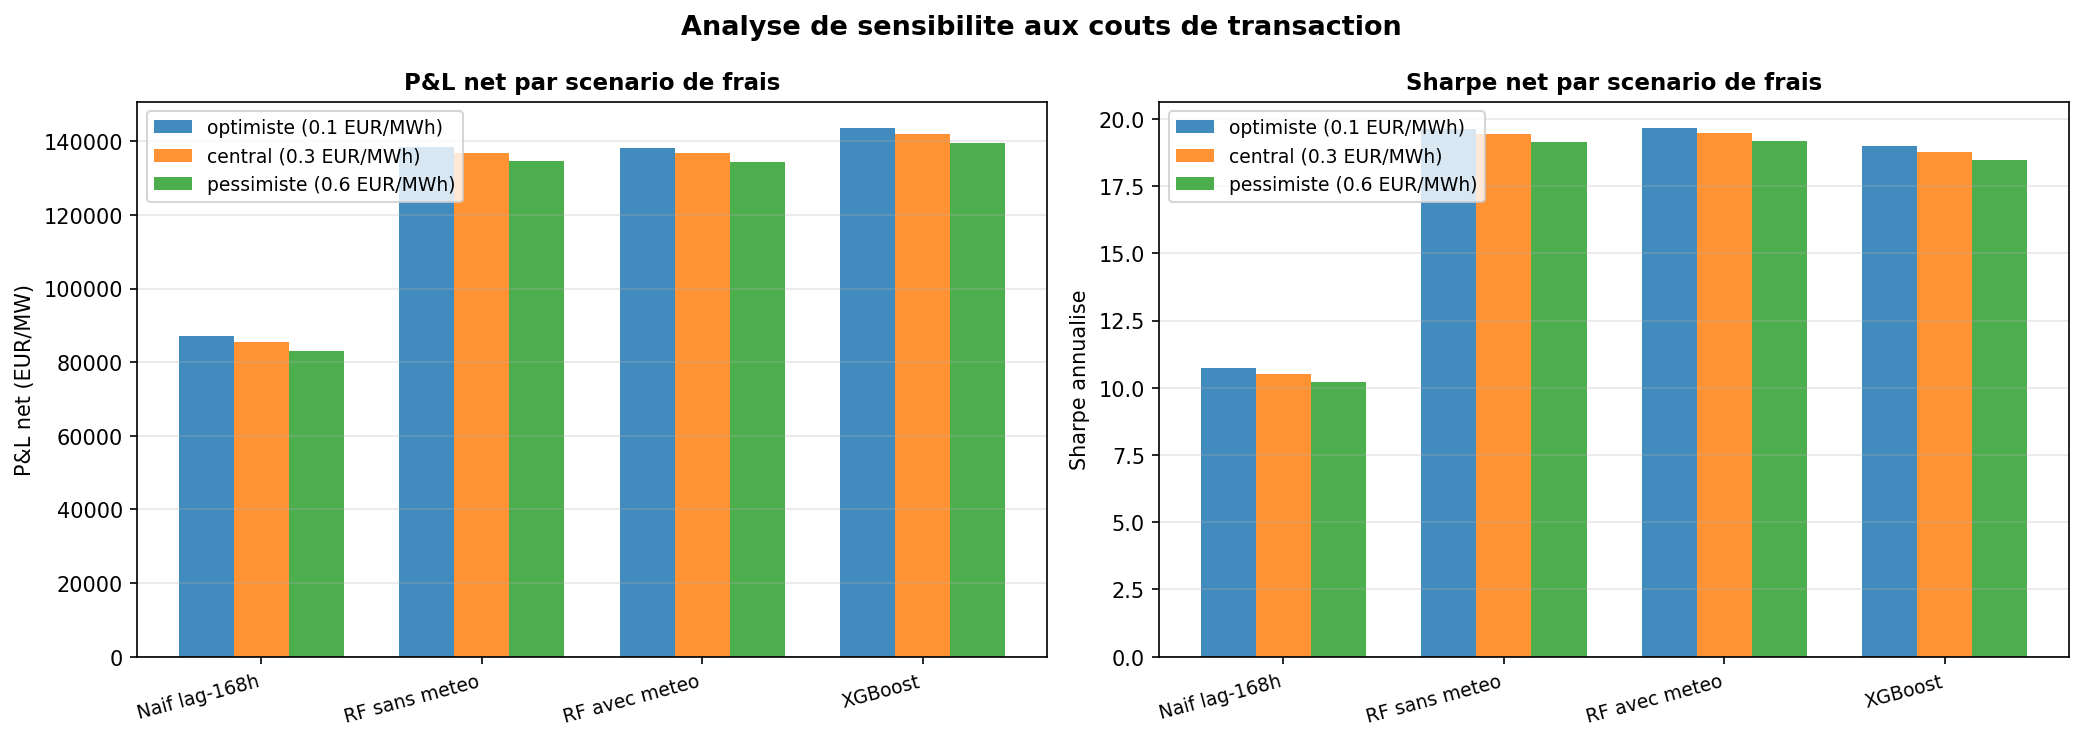
\includegraphics[width=\textwidth]{cost_sensitivity.png}
  \caption{Net P\&L (left) and Sharpe (right) by model and transaction cost scenario. All ML models remain substantially profitable even under the pessimistic cost assumption.}
  \label{fig:cost_sensitivity}
\end{figure}

\section{Methodological Limitations}

We document three limitations that should be considered when interpreting the backtest results:

\begin{enumerate}
  \item \textbf{Short test window:} The test period covers 12 months of a single market regime (normalised post-crisis prices). Generalising these results to other regimes — including the 2022 crisis or future periods of structural change — requires additional testing.

  \item \textbf{Perfect execution assumed:} The backtest assumes that all bids are matched at the clearing price without slippage. In practice, large positions may affect the clearing price, and partial fills may occur during low-liquidity hours.

  \item \textbf{Note on Sharpe interpretation:} The Sharpe ratios reported (10--19 annualised on daily P\&L) should not be compared to equity fund benchmarks. Electricity markets operate with a different risk-return structure: prices are highly mean-reverting at long horizons (the long-only earns zero), the market is less competitive than equity markets, and the strategy operates at 1 MW with no leverage. The relevant comparison is between models, not to absolute Sharpe thresholds from other asset classes.
\end{enumerate}

% ============================================================
%  Chapter 6 — Discussion
% ============================================================
\chapter{Discussion}
\label{chap:discussion}

\section{The Central Finding: Weather Is Regime-Dependent}

The thesis's primary empirical contribution is a finding with two parts that
must be understood together. In the stable 2024--25 test period, weather
features add no statistically significant forecast improvement over a
fundamental-only Random Forest ($p = 0.572$, DM = $-0.565$). In the 2022
energy crisis, the same comparison yields $p < 0.001$ (DM = $-13.27$):
weather is highly significant. The role of weather in French day-ahead
electricity price forecasting is therefore not a binary yes/no question but a
function of market regime.

This result reconciles apparently contradictory intuitions. Weather obviously
drives electricity demand and renewable supply, so one would expect it to
matter for price forecasting. Yet in a market where price-setting fundamentals
(TTF gas, nuclear availability) are explicitly modelled, weather information
may be fully subsumed. The resolution is that the degree of subsumption depends
on how tight the coupling between weather and fundamentals is — and this
coupling changes under stress.

\subsection{The Information Redundancy Hypothesis}

We argue that in stable market conditions, weather information is already
embedded in other features of the model through three distinct channels:

\textbf{Load forecast as a temperature proxy.} RTE publishes an hourly load
forecast for D+1 that is computed using a proprietary model incorporating
temperature forecasts \citep{rte2023}. When we include this load forecast in
the feature matrix, we implicitly condition on a temperature-adjusted demand
estimate. The raw temperature variable then adds no marginal information beyond
what is already captured by RTE's own weather-informed demand forecast. The
high correlation between HDD and load forecast ($r > 0.60$, visible in
Figure~\ref{fig:corr_matrix}) confirms this redundancy.

\textbf{TTF gas price as an energy weather proxy.} European gas prices respond
to heating demand aggregated across all gas-consuming countries. A cold spell
in France simultaneously increases French electricity demand and increases gas
demand across Europe, pushing TTF higher. A model that includes TTF therefore
already incorporates a pan-European temperature signal through the lens of the
commodity market. This indirect transmission channel reflects a well-established principle: commodity
markets aggregate weather information efficiently when the weather-commodity
relationship is stable.

\textbf{Nuclear availability dominance.} In France, the availability of the
nuclear fleet explains a disproportionate share of price variance relative to
other European markets. In 2022, nuclear availability fell to $\approx$40\%,
creating price variance that no weather feature can explain (the outages were
driven by corrosion-related technical failures, not weather). With nuclear
availability as an explicit feature, the model's residual variance is already
low in stable conditions, leaving little room for weather variables to
contribute further.

\subsection{Why the Crisis Breaks Redundancy}

The 2022 result ($p < 0.001$) reveals that the information redundancy is
not unconditional. Three mechanisms can explain why weather becomes significant
in a crisis regime:

\textbf{Decoupling of TTF and local temperature.} During the 2021--2023 gas
supply crisis, TTF prices were predominantly driven by geopolitical supply
shocks (Russian gas curtailments) rather than weather. The normal correlation
between cold temperatures and TTF rises was disrupted: prices were high
regardless of the weather. In this environment, the residual temperature effect
on electricity demand could not be subsumed by TTF — it had to be captured
by the raw temperature variable directly. The information redundancy broke down
because the mediating variable (TTF) lost its weather signal.

\textbf{Nuclear constraint amplification.} With nuclear availability at 40\%,
France had limited buffer capacity to absorb demand surges driven by cold
weather. In normal conditions (nuclear at 70\%), a cold spell adds demand that
nuclear can partially accommodate; with nuclear severely constrained, the same
cold spell forces much higher dispatch of expensive gas and oil peakers,
amplifying the price response. This non-linear amplification makes the direct
temperature-price channel visible in the data.

\textbf{Higher signal-to-noise ratio.} The 2022 crisis produced extreme price
levels that created larger absolute prediction errors, but also larger
differences between Model B and Model C: even a small absolute MAE improvement
(0.73 EUR/MWh) is detectable by the DM test at the high absolute price levels
of 2022. The test's statistical power to detect a given proportional effect
is higher when the loss differential has a larger mean.

\subsection{Implications for Forecasting Practice}

This finding has concrete practical implications:

\textit{Stable markets:} Building a rich fundamental model that includes
cross-border flows, fuel prices, and nuclear availability is sufficient to
capture the weather signal implicitly in the French market. The additional cost
and complexity of integrating real-time weather forecasts from ERA5 or NWP
models may not be justified, provided that the load forecast and fuel price
data are available. This lowers the barrier to entry for model builders
without proprietary meteorological data infrastructure.

\textit{Crisis markets:} When TTF-temperature co-movement decouples (e.g.,
during geopolitical supply shocks) or when nuclear availability is severely
constrained, weather features provide statistically and economically significant
value. Market participants entering production forecasting should build
weather-aware models as a contingency, even if weather features are switched off
during normal regimes. A regime-switching model that activates or de-weights
weather features based on nuclear availability and TTF volatility is a
promising direction for future work.

\textit{Cross-market applicability:} This result may not generalise to markets
with higher renewable penetration. In Germany, renewables accounted for over 60\% of electricity generation in 2024
(Fraunhofer ISE, 2025), with wind and solar jointly representing close to half of
all generation, and the direct impact of weather on supply is much larger.
The indirect TTF channel is less likely to fully capture the wind-solar
generation effect in Germany than in France, suggesting that weather features
would be more valuable in the German market context. Testing this hypothesis
in a comparative France-Germany study is a natural extension.

\section{XGBoost Underperformance and Its Implications}

The underperformance of XGBoost (Model D) relative to Random Forest (Models B
and C) is a secondary finding that deserves careful interpretation. With our
hyperparameters, XGBoost achieves MAE of 19.14 EUR/MWh and R$^2$ of 0.659 in
the stable period, compared to approximately 16.94 EUR/MWh and 0.776 for the
Random Forests. In the 2022 crisis, the gap widens further (76.32 vs 66.55
EUR/MWh). Two factors explain this pattern.

First, XGBoost's sequential boosting mechanism assigns higher weight to
poorly-fitted observations in each iteration. In the presence of genuine
outliers driven by extraordinary events (the 2022 nuclear-gas crisis), this
can lead to overfitting on crisis-era residuals at the expense of
normal-market performance. Random Forests average over bootstrap samples,
which is more robust to distributional shifts across regimes.

Second, the hyperparameters used here (500 estimators, $\eta = 0.05$, max
depth 6) were chosen to be reasonable defaults but were not tuned to the
specific loss landscape of our data. The Random Forest's hyperparameters
(500 trees, max depth 10, min leaf 5) were similarly not optimised, but RF
is known to be less sensitive to hyperparameter choice than XGBoost, whose
performance depends more critically on the learning rate, regularisation
terms ($\lambda$, $\alpha$), and subsampling rates. A Bayesian hyperparameter
search with time-series cross-validation could plausibly close or reverse the
performance gap between XGBoost and RF, and is a priority for future work.

The implication for practitioners is that the comparison between RF and
XGBoost reported here should \textit{not} be interpreted as evidence that RF
is inherently superior to boosted trees for electricity price forecasting. The
result reflects our specific configuration. The comparison between Model B and
Model C (RF with vs without weather), however, is robust: both models use the
same architecture and differ only in the feature set, making the DM test a
clean ablation study.

\section{Limitations}
\label{sec:limitations}

\subsection{Static Model and Distribution Shift}

Both RF and XGBoost are trained once on data from 2018--2024 and applied
without retraining to the test period. The training set includes the 2022 crisis
regime, while the test set covers a normalised post-crisis regime. In principle,
the model trained on crisis-level prices (occasionally exceeding 1{,}000
EUR/MWh) may not generalise optimally to a test regime where prices rarely
exceed 200 EUR/MWh. A walk-forward expanding-window retraining scheme — in
which the model is retrained monthly using all data available up to that point
— would provide a more realistic assessment of production performance and is
a prerequisite for operational deployment.

\subsection{Price Spike Forecasting}

Both models systematically underestimate extreme price events. During the
test period, hours with prices above 200 EUR/MWh contribute disproportionately
to RMSE despite representing fewer than 1\% of observations. Point forecasting
models trained on MAE or RMSE loss functions target the conditional mean, which
is pulled toward the bulk of the distribution. Dedicated spike detection
approaches — including two-stage models (a classifier for spike probability
followed by a spike magnitude regression) or quantile regression forests for
prediction intervals — could substantially improve tail performance. This is
particularly important for risk management applications where exposure to
extreme hours drives the economic value of the forecast.

\subsection{Negative Price Dynamics}

Negative prices represent approximately 3--8\% of hours in recent years
(Figure~\ref{fig:price_dist}). Our sMAPE metric handles negative prices
correctly, but the RF models may not accurately represent the specific dynamics
of price formation below zero, where the mechanism shifts from demand-driven
to supply-push (inflexible generators paying consumers to absorb excess
generation). A dedicated modelling approach for the negative-price regime is
a natural extension.

\subsection{Missing EU ETS Carbon Allowances}

EU ETS carbon allowance prices (EUA) were not included as a standalone feature.
EUA prices directly raise the operating cost of gas and coal generation through
the carbon component of the generation cost. Their exclusion may reduce the
model's accuracy during periods of high carbon price volatility, which have
coincided with some of the most extreme electricity price episodes (2021--2022).
The TTF-coal spread partially proxies for EUA (as all three series moved
together during the crisis), but a more complete fundamental model would include
EUA explicitly.

\subsection{Single Out-of-Sample Regime}

The main test period (May 2024--April 2025) covers only one market regime.
The 2022 robustness exercise provides an important second data point, but does
not constitute a full walk-forward evaluation. The reliability of the
statistical conclusions would be strengthened by testing on additional
out-of-sample windows covering different nuclear availability levels, renewable
penetration levels, and geopolitical conditions.

\section{Future Research Directions}

\begin{enumerate}
  \item \textbf{Regime-switching weather model:} Building an explicit
  regime-switching mechanism that activates weather features when nuclear
  availability falls below a threshold (e.g., 0.55) or when TTF volatility
  exceeds a threshold, combining the efficiency of the fundamental model in
  stable regimes with the accuracy of the weather-augmented model in stress
  regimes.

  \item \textbf{Probabilistic forecasting:} Replace point forecasts with
  prediction intervals or full predictive distributions using Quantile
  Regression Forests or conformal prediction. Probabilistic forecasts are
  increasingly demanded by market participants for option pricing and risk
  management.

  \item \textbf{Comparative France--Germany study:} Test whether weather
  features are more significant in Germany, where renewable penetration is
  substantially higher and the indirect TTF-weather channel is less dominant.
  Such a comparison would directly test our information redundancy hypothesis
  in a different market structure.

  \item \textbf{XGBoost hyperparameter optimisation:} A systematic Bayesian
  search with temporal cross-validation, using a custom time-aware split
  strategy (e.g., 6-fold expanding window), could close the performance gap
  between XGBoost and RF.

  \item \textbf{Transformer and LSTM architectures:} Long Short-Term Memory
  networks and Transformer-based models have demonstrated promise on energy
  time series with long-range dependencies \citep{lago2018}. Comparing these
  to our RF baseline within the same experimental framework — including the
  same DM test procedure — would be a natural extension.
\end{enumerate}

% ============================================================
%  Chapter 7 — Conclusion
% ============================================================
\chapter{Conclusion}
\label{chap:conclusion}

\section{Summary of Findings}

This thesis investigated whether weather variables significantly improve day-ahead electricity price forecasting for the French market, and whether the resulting forecasts generate economic value through a directional trading strategy. Our analysis, conducted on a comprehensive hourly dataset spanning January 2018 to April 2025, leads to four principal conclusions.

\textbf{First, machine learning models substantially outperform the na\"{i}ve benchmark.} Both Random Forest variants reduce MAE by approximately 49\% (from 33.09 to $\approx$16.94 EUR/MWh) and increase R$^2$ from 0.16 to 0.78 on the out-of-sample test set (May 2024--April 2025). The Diebold-Mariano test confirms this improvement is highly statistically significant ($p < 0.001$). The performance is robust: both RF models record positive monthly Sharpe ratios in every month of the test period.

\textbf{Second, the role of weather is regime-dependent.} In the stable
May 2024--April 2025 test period, weather features produce no statistically
significant forecast improvement ($p = 0.572$, DM $= -0.565$). However, a
validation on the 2022 energy crisis reverses this result: the DM test yields
$p < 0.001$ (DM $= -13.27$), and Model C reduces MAE by 0.73 EUR/MWh over
Model B in 2022. We attribute the stable-period non-significance to the
\textit{information redundancy hypothesis}: the load forecast, TTF gas price,
and nuclear availability ratio already encode the meteorological information
relevant to French price formation under normal conditions. The significance
in 2022 arises because the gas supply crisis decoupled TTF from local
temperature, breaking the indirect weather channel and making the direct
temperature-demand effect visible. This regime-dependent finding is the thesis's
primary empirical contribution and calls for nuanced interpretation: weather
features are neither always beneficial nor always redundant — their value
depends on the structural state of the gas and nuclear supply.

\textbf{Third, Random Forest outperforms XGBoost with default hyperparameters.} XGBoost achieves a higher absolute P\&L in the backtest but at the cost of a Maximum Drawdown more than three times larger than the Random Forest. On a risk-adjusted basis (Calmar ratio of 107 vs 320--328), RF is the superior model. The performance gap is attributed to XGBoost's sensitivity to extreme price observations in the training set and could be closed through systematic hyperparameter optimisation.

\textbf{Fourth, the forecasting models generate economically significant value.} Under the central transaction cost scenario (0.30 EUR/MWh), RF models generate net P\&L of approximately 136,700 EUR/MW over the 12-month test period, compared to 85,500 for the na\"{i}ve and essentially zero for the long-only reference. The trading performance is robust to cost assumptions (cost drag below 2\% across scenarios) and consistent across all calendar months.

\section{Recommendations}

Based on our findings, we offer the following recommendations for practitioners:

\begin{itemize}
  \item \textbf{Use Random Forest as the primary forecasting model} for the French day-ahead market. It outperforms both the na\"{i}ve benchmark and XGBoost on risk-adjusted metrics, and its MDI feature importances provide interpretable insights into price drivers.

  \item \textbf{Prioritise fundamental features in stable regimes; retain weather capability for crisis regimes.} Under normal market conditions, model development effort is better spent improving the quality of load forecasts, fuel price integration, and cross-border flow data rather than adding more meteorological variables. However, the 2022 result demonstrates that weather features provide statistically significant value during crisis regimes characterised by low nuclear availability and decoupled gas-weather co-movement. A production model should include weather features with a regime-detection mechanism that activates or de-weights them based on observable market conditions.

  \item \textbf{Implement periodic retraining.} The current static model is trained through April 2024. A monthly or quarterly retraining schedule would adapt to structural market changes (increasing renewable penetration, nuclear fleet evolution) and is a prerequisite for production deployment.

  \item \textbf{Complement point forecasts with prediction intervals.} The high RMSE relative to MAE indicates the presence of large forecast errors during spike periods. Risk managers should complement model predictions with scenario analysis for extreme price events.
\end{itemize}

\section{Broader Implications}

The regime-dependent weather finding reflects a broader insight about
information aggregation in commodity markets. In stable conditions, when market
prices (TTF gas) and operational forecasts (RTE load forecast) already
incorporate weather expectations, raw meteorological variables become
statistically redundant. This principle — that feature selection should account
for the information already embedded in price-based variables — is likely
applicable beyond the electricity market to other commodity forecasting
problems. However, the 2022 result shows that this redundancy is conditional:
structural supply shocks that break the normal co-movement between commodity
prices and weather can reinstate the direct weather channel. Forecasters should
monitor the stability of these co-movement relationships and treat weather
feature inclusion as a dynamic decision rather than a permanent design choice.

From a market design perspective, this thesis illustrates how the quality of
publicly available data (ENTSO-E generation data, RTE load forecasts) can
substitute for proprietary weather modelling infrastructure during normal market
conditions, lowering the barriers to participation in day-ahead electricity
price forecasting. During crisis regimes, however, direct weather integration
provides measurable value that cannot be obtained from public market data alone.

\section{Code and Data Availability}

The complete codebase for this thesis — including data collection pipelines (ENTSO-E API, ERA5 CDS API, fuel prices), feature engineering, model training, evaluation, and the trading backtest — is available upon request. Data from ENTSO-E and ERA5 are publicly available under their respective open data licences.


% ── Bibliography ─────────────────────────────────────────────
\bibliographystyle{apalike}
\bibliography{bibliography}

% ── Appendix ─────────────────────────────────────────────────
\begin{appendices}
\chapter{Model Hyperparameters}
\label{app:hyperparams}

\begin{table}[H]
\centering
\caption{Hyperparameters for Random Forest (Models B and C)}
\begin{tabular}{ll}
\toprule
\textbf{Parameter} & \textbf{Value} \\
\midrule
n\_estimators   & 500 \\
max\_depth      & 10  \\
min\_samples\_leaf & 5 \\
max\_features   & \texttt{sqrt} \\
n\_jobs         & $-1$ (all cores) \\
random\_state   & 42 \\
\bottomrule
\end{tabular}
\end{table}

\begin{table}[H]
\centering
\caption{Hyperparameters for XGBoost (Model D)}
\begin{tabular}{ll}
\toprule
\textbf{Parameter} & \textbf{Value} \\
\midrule
n\_estimators     & 500 \\
learning\_rate    & 0.05 \\
max\_depth        & 6 \\
subsample         & 0.8 \\
colsample\_bytree & 0.8 \\
random\_state     & 42 \\
\bottomrule
\end{tabular}
\end{table}

\chapter{Full Feature List}
\label{app:features}

\begin{table}[H]
\centering
\small
\caption{Complete list of features used in Models B, C and D}
\begin{tabularx}{\textwidth}{llX}
\toprule
\textbf{Category} & \textbf{Feature} & \textbf{Description} \\
\midrule
\multirow{5}{*}{Calendar}
  & hour\_sin / hour\_cos   & Sine/cosine encoding of hour of day \\
  & month\_sin / month\_cos & Sine/cosine encoding of month \\
  & dayofweek              & Day of week (0=Monday) \\
  & is\_weekend            & Binary weekend indicator \\
\midrule
\multirow{5}{*}{Price lags}
  & price\_lag24h          & Price 24 hours ago \\
  & price\_lag48h          & Price 48 hours ago \\
  & price\_lag168h         & Price 168 hours ago (same hour, previous week) \\
  & price\_roll24h\_mean   & 24-hour rolling mean (lagged 24h) \\
  & price\_roll168h\_mean  & 168-hour rolling mean (lagged 24h) \\
\midrule
\multirow{7}{*}{Fundamentals}
  & load\_forecast\_mw      & Hourly load forecast (MW) \\
  & gen\_nuclear\_mw        & Nuclear generation (MW) \\
  & gen\_gas\_mw            & Gas generation (MW) \\
  & gen\_hydro\_ror\_mw     & Run-of-river hydro generation (MW) \\
  & gen\_hydro\_reservoir\_mw & Reservoir hydro generation (MW) \\
  & gen\_solar\_mw          & Solar generation (MW) \\
  & gen\_wind\_onshore\_mw  & Onshore wind generation (MW) \\
\midrule
\multirow{4}{*}{Cross-border}
  & flow\_net\_fr\_de\_mw  & Net cross-border flow France--Germany (MW) \\
  & flow\_net\_fr\_es\_mw  & Net cross-border flow France--Spain (MW) \\
  & flow\_net\_fr\_gb\_mw  & Net cross-border flow France--UK (MW) \\
  & flow\_net\_fr\_be\_mw  & Net cross-border flow France--Belgium (MW) \\
\midrule
\multirow{2}{*}{Fuel prices}
  & ttf\_eur\_mwh          & TTF natural gas day-ahead price (EUR/MWh) \\
  & coal\_eur\_t           & ARA coal price (EUR/tonne) \\
\midrule
\multirow{6}{*}{Weather}
  & temperature\_2m        & 2m air temperature, spatial mean France (\textdegree C) \\
  & wind\_speed\_10m       & 10m wind speed (m/s) \\
  & solar\_radiation       & Surface solar irradiance (W/m\textsuperscript{2}) \\
  & precipitation          & Total precipitation (m/h) \\
  & hdd                    & Heating Degree Days (threshold 17\textdegree C, RTE) \\
  & cdd                    & Cooling Degree Days (threshold 22\textdegree C) \\
\midrule
\multirow{3}{*}{Derived}
  & wind\_power\_proxy     & Wind speed$^3$ (proportional to wind power) \\
  & weather\_stress\_index & HDD / wind speed (cold \& low wind composite) \\
  & nuclear\_avail\_ratio  & Nuclear generation / 63,000 MW installed capacity \\
\bottomrule
\end{tabularx}
\end{table}

\end{appendices}

\end{document}
